%% 由 build/emit_tex.py 生成（生成物，勿手改）；定制请放 user_style.tex / user_meta.yaml
\chapter{Sklearn及其基本使用}\label{sklearnux53caux5176ux57faux672cux4f7fux7528}

\section{01
数据集的预处理}\label{ux6570ux636eux96c6ux7684ux9884ux5904ux7406}

\begin{quote}
本节是从``原始数据''到``可训练数据''的第一步：特征编码、特征缩放、数据集切分、交叉验证与特征选择。所有代码在
sklearn 1.6.1、Python 3.13 下运行验证。
\end{quote}

\subsection{本节目标}\label{ux672cux8282ux76eeux6807-21}

\begin{enumerate}
\def\labelenumi{\arabic{enumi}.}
\tightlist
\item
  会用 \texttt{OneHotEncoder} / \texttt{LabelEncoder}
  处理分类特征，并说清两者适用场景。
\item
  会用 \texttt{StandardScaler} / \texttt{MinMaxScaler} 缩放连续特征。
\item
  会用 \texttt{train\_test\_split} 切分数据，并用
  \texttt{cross\_val\_score} / \texttt{LeaveOneOut} 做交叉验证。
\item
  会用
  \texttt{VarianceThreshold}、\texttt{SelectKBest}、\texttt{RFE}、\texttt{Lasso}、\texttt{SelectFromModel}
  做特征选择。
\item
  理解预处理必须放在 Pipeline 中，避免数据泄漏。
\end{enumerate}

\subsection{先修}\label{ux5148ux4fee-21}

\begin{itemize}
\tightlist
\item
  NumPy 数组操作、Pandas 基本用法（第 1、4 章）。
\item
  了解``均值/方差/相关系数''与``特征量纲''概念。
\end{itemize}

\subsection{官方文档 /
参考入口}\label{ux5b98ux65b9ux6587ux6863-ux53c2ux8003ux5165ux53e3-7}

\begin{itemize}
\tightlist
\item
  sklearn
  预处理：https://scikit-learn.org/stable/modules/preprocessing.html
\item
  sklearn
  模型选择：https://scikit-learn.org/stable/modules/cross\_validation.html
\item
  sklearn
  特征选择：https://scikit-learn.org/stable/modules/feature\_selection.html
\item
  sklearn 数据分割
  API：https://scikit-learn.org/stable/modules/generated/sklearn.model\_selection.train\_test\_split.html
\end{itemize}

\subsection{正文}\label{ux6b63ux6587}

\subsubsection{1.
特征编码：把``文字''变成``数字''}\label{ux7279ux5f81ux7f16ux7801ux628aux6587ux5b57ux53d8ux6210ux6570ux5b57}

大多数 sklearn 模型只能吃数值矩阵。对待分类特征，有两种常见编码。

\paragraph{1.1
独热编码（OneHotEncoder）}\label{ux72ecux70edux7f16ux7801onehotencoder}

把每个类别展开成一位为 1、其余为 0 的向量。默认输出稀疏矩阵，用
\texttt{sparse\_output=False} 得到稠密数组。

\begin{Shaded}
\begin{Highlighting}[]
\ImportTok{import}\NormalTok{ numpy }\ImportTok{as}\NormalTok{ np}
\ImportTok{from}\NormalTok{ sklearn.preprocessing }\ImportTok{import}\NormalTok{ OneHotEncoder}

\NormalTok{data }\OperatorTok{=}\NormalTok{ np.array([[}\StringTok{\textquotesingle{}male\textquotesingle{}}\NormalTok{], [}\StringTok{\textquotesingle{}female\textquotesingle{}}\NormalTok{], [}\StringTok{\textquotesingle{}male\textquotesingle{}}\NormalTok{], [}\StringTok{\textquotesingle{}female\textquotesingle{}}\NormalTok{]])}
\NormalTok{encoder }\OperatorTok{=}\NormalTok{ OneHotEncoder(sparse\_output}\OperatorTok{=}\VariableTok{False}\NormalTok{)}
\NormalTok{encoded }\OperatorTok{=}\NormalTok{ encoder.fit\_transform(data)}
\BuiltInTok{print}\NormalTok{(}\StringTok{"categories\_:"}\NormalTok{, encoder.categories\_)}
\BuiltInTok{print}\NormalTok{(}\StringTok{"shape:"}\NormalTok{, encoded.shape)}
\BuiltInTok{print}\NormalTok{(}\StringTok{"特征名:"}\NormalTok{, encoder.get\_feature\_names\_out())}
\BuiltInTok{print}\NormalTok{(encoded)}
\end{Highlighting}
\end{Shaded}

\begin{Shaded}
\begin{Highlighting}[]
\NormalTok{categories\_: [array([\textquotesingle{}female\textquotesingle{}, \textquotesingle{}male\textquotesingle{}], dtype=\textquotesingle{}\textless{}U6\textquotesingle{})]}
\NormalTok{shape: (4, 2)}
\NormalTok{特征名: [\textquotesingle{}x0\_female\textquotesingle{} \textquotesingle{}x0\_male\textquotesingle{}]}
\NormalTok{[[0. 1.]}
\NormalTok{ [1. 0.]}
\NormalTok{ [0. 1.]}
\NormalTok{ [1. 0.]]}
\end{Highlighting}
\end{Shaded}

\begin{quote}
注意：\texttt{male} 被编码为 \texttt{{[}0,1{]}}（因为
\texttt{categories\_} 按字母序把 \texttt{female} 排在 0
列、\texttt{male} 排 1
列）。独热编码没有``谁大谁小''的含义，适合无序类别。
\end{quote}

\paragraph{1.2
标签编码（LabelEncoder）}\label{ux6807ux7b7eux7f16ux7801labelencoder}

把每个类别映射成 0、1、2
等整数。它暗示类别之间有顺序，对无序类别（如颜色、性别）通常不合适。

\begin{Shaded}
\begin{Highlighting}[]
\ImportTok{from}\NormalTok{ sklearn.preprocessing }\ImportTok{import}\NormalTok{ LabelEncoder}

\NormalTok{labels }\OperatorTok{=}\NormalTok{ [}\StringTok{\textquotesingle{}male\textquotesingle{}}\NormalTok{, }\StringTok{\textquotesingle{}female\textquotesingle{}}\NormalTok{, }\StringTok{\textquotesingle{}male\textquotesingle{}}\NormalTok{, }\StringTok{\textquotesingle{}female\textquotesingle{}}\NormalTok{]}
\NormalTok{le }\OperatorTok{=}\NormalTok{ LabelEncoder().fit(labels)}
\BuiltInTok{print}\NormalTok{(}\StringTok{"classes\_:"}\NormalTok{, le.classes\_)}
\BuiltInTok{print}\NormalTok{(}\StringTok{"transform:"}\NormalTok{, le.transform(labels))}
\end{Highlighting}
\end{Shaded}

\begin{Shaded}
\begin{Highlighting}[]
\NormalTok{classes\_: [\textquotesingle{}female\textquotesingle{} \textquotesingle{}male\textquotesingle{}]}
\NormalTok{transform: [1 0 1 0]}
\end{Highlighting}
\end{Shaded}

\begin{quote}
若类别本身有序（如 \texttt{小/中/大}），可改用 \texttt{OrdinalEncoder}
并显式指定 \texttt{categories}；若只是把字符串标签喂给分类器，常用
\texttt{LabelEncoder} 只看目标 y，而特征 x 的分类列建议用
\texttt{OneHotEncoder} 或 \texttt{OrdinalEncoder}。
\end{quote}

\subsubsection{2.
特征缩放：把量纲拉平}\label{ux7279ux5f81ux7f29ux653eux628aux91cfux7eb2ux62c9ux5e73}

当各列量纲差别很大（比如一列在 0\textasciitilde1，另一列在 10\^{}4
量级）时，距离类算法（KNN、SVM、KMeans、PCA）会被大方差特征主导，因此需要缩放。

\paragraph{2.1
标准化（StandardScaler）}\label{ux6807ux51c6ux5316standardscaler}

\texttt{x\textquotesingle{}\ =\ (x\ -\ mean)\ /\ std}，使每列均值
0、标准差 1。

\begin{Shaded}
\begin{Highlighting}[]
\ImportTok{import}\NormalTok{ numpy }\ImportTok{as}\NormalTok{ np}
\ImportTok{from}\NormalTok{ sklearn.preprocessing }\ImportTok{import}\NormalTok{ StandardScaler}

\NormalTok{X }\OperatorTok{=}\NormalTok{ np.array([[}\DecValTok{1}\NormalTok{, }\DecValTok{2}\NormalTok{], [}\DecValTok{3}\NormalTok{, }\DecValTok{4}\NormalTok{], [}\DecValTok{5}\NormalTok{, }\DecValTok{6}\NormalTok{]])}
\NormalTok{ss }\OperatorTok{=}\NormalTok{ StandardScaler().fit(X)}
\BuiltInTok{print}\NormalTok{(}\StringTok{"mean\_:"}\NormalTok{, ss.mean\_, }\StringTok{"scale\_:"}\NormalTok{, np.}\BuiltInTok{round}\NormalTok{(ss.scale\_, }\DecValTok{6}\NormalTok{))}
\BuiltInTok{print}\NormalTok{(ss.transform(X))}
\end{Highlighting}
\end{Shaded}

\begin{Shaded}
\begin{Highlighting}[]
\NormalTok{mean\_: [3. 4.] scale\_: [1.632993 1.632993]}
\NormalTok{[[{-}1.22474487 {-}1.22474487]}
\NormalTok{ [ 0.          0.        ]}
\NormalTok{ [ 1.22474487  1.22474487]]}
\end{Highlighting}
\end{Shaded}

\paragraph{2.2
归一化（MinMaxScaler）}\label{ux5f52ux4e00ux5316minmaxscaler}

把每列压缩到 \texttt{{[}0,\ 1{]}}（或其他 \texttt{feature\_range}）。

\begin{Shaded}
\begin{Highlighting}[]
\ImportTok{from}\NormalTok{ sklearn.preprocessing }\ImportTok{import}\NormalTok{ MinMaxScaler}

\NormalTok{mm }\OperatorTok{=}\NormalTok{ MinMaxScaler().fit(X)}
\BuiltInTok{print}\NormalTok{(}\StringTok{"data\_min\_:"}\NormalTok{, mm.data\_min\_, }\StringTok{"data\_max\_:"}\NormalTok{, mm.data\_max\_)}
\BuiltInTok{print}\NormalTok{(mm.transform(X))}
\end{Highlighting}
\end{Shaded}

\begin{Shaded}
\begin{Highlighting}[]
\NormalTok{data\_min\_: [1. 2.] data\_max\_: [5. 6.]}
\NormalTok{[[0.  0. ]}
\NormalTok{ [0.5 0.5]}
\NormalTok{ [1.  1. ]]}
\end{Highlighting}
\end{Shaded}

\begin{quote}
标准化对异常值更稳健（用均值/标准差），归一化把数据严格限制到区间。若有人告诉你``某个算法必须归一化''，指的是这两者之一；具体选哪个要看数据分布与模型（树模型一般不需要缩放）。
\end{quote}

\subsubsection{3.
数据集切分与交叉验证}\label{ux6570ux636eux96c6ux5207ux5206ux4e0eux4ea4ux53c9ux9a8cux8bc1}

\paragraph{3.1 train\_test\_split}\label{train_test_split}

\begin{Shaded}
\begin{Highlighting}[]
\ImportTok{from}\NormalTok{ sklearn.model\_selection }\ImportTok{import}\NormalTok{ train\_test\_split}
\ImportTok{from}\NormalTok{ sklearn.datasets }\ImportTok{import}\NormalTok{ load\_iris}

\NormalTok{iris }\OperatorTok{=}\NormalTok{ load\_iris()}\OperatorTok{;}\NormalTok{ X, y }\OperatorTok{=}\NormalTok{ iris.data, iris.target}
\NormalTok{Xtr, Xte, ytr, yte }\OperatorTok{=}\NormalTok{ train\_test\_split(X, y, test\_size}\OperatorTok{=}\FloatTok{0.3}\NormalTok{, random\_state}\OperatorTok{=}\DecValTok{42}\NormalTok{, stratify}\OperatorTok{=}\NormalTok{y)}
\BuiltInTok{print}\NormalTok{(}\StringTok{"train shape:"}\NormalTok{, Xtr.shape, }\StringTok{"test shape:"}\NormalTok{, Xte.shape)}
\BuiltInTok{print}\NormalTok{(}\StringTok{"测试集各类数量:"}\NormalTok{, np.unique(yte, return\_counts}\OperatorTok{=}\VariableTok{True}\NormalTok{))}
\end{Highlighting}
\end{Shaded}

\begin{Shaded}
\begin{Highlighting}[]
\NormalTok{train shape: (105, 4) test shape: (45, 4)}
\NormalTok{测试集各类数量: (array([0, 1, 2]), array([15, 15, 15]))}
\end{Highlighting}
\end{Shaded}

\begin{quote}
\texttt{stratify=y}
让训练/测试集各类比例一致（对分类很重要）；\texttt{random\_state=42}
保证可复现。
\end{quote}

\paragraph{3.2 K
折交叉验证（cross\_val\_score）}\label{k-ux6298ux4ea4ux53c9ux9a8cux8bc1cross_val_score}

把数据切成 K 份，轮流用 K-1 份训练、1 份测试，最后平均各折分数。

\begin{Shaded}
\begin{Highlighting}[]
\ImportTok{from}\NormalTok{ sklearn.linear\_model }\ImportTok{import}\NormalTok{ LogisticRegression}
\ImportTok{from}\NormalTok{ sklearn.model\_selection }\ImportTok{import}\NormalTok{ cross\_val\_score}

\NormalTok{model }\OperatorTok{=}\NormalTok{ LogisticRegression(max\_iter}\OperatorTok{=}\DecValTok{1000}\NormalTok{)}
\NormalTok{scores }\OperatorTok{=}\NormalTok{ cross\_val\_score(model, Xtr, ytr, cv}\OperatorTok{=}\DecValTok{5}\NormalTok{)}
\BuiltInTok{print}\NormalTok{(}\StringTok{"各折分数:"}\NormalTok{, np.}\BuiltInTok{round}\NormalTok{(scores, }\DecValTok{4}\NormalTok{))}
\BuiltInTok{print}\NormalTok{(}\StringTok{"平均:"}\NormalTok{, }\BuiltInTok{round}\NormalTok{(scores.mean(), }\DecValTok{4}\NormalTok{))}
\end{Highlighting}
\end{Shaded}

\begin{Shaded}
\begin{Highlighting}[]
\NormalTok{各折分数: [0.9524 0.9524 1.     0.9524 1.    ]}
\NormalTok{平均: 0.9714}
\end{Highlighting}
\end{Shaded}

\begin{quote}
\texttt{cross\_val\_score} 内部会把每个模型 \texttt{fit}
在训练折、\texttt{score} 在验证折，因此它比单次 train/test
更稳健、也更少受随机划分影响。
\end{quote}

\paragraph{3.3
留一交叉验证（LeaveOneOut）}\label{ux7559ux4e00ux4ea4ux53c9ux9a8cux8bc1leaveoneout}

每次只留 1 个样本测试。适合小数据集，但计算量大。

\begin{Shaded}
\begin{Highlighting}[]
\ImportTok{from}\NormalTok{ sklearn.model\_selection }\ImportTok{import}\NormalTok{ LeaveOneOut}

\NormalTok{loo }\OperatorTok{=}\NormalTok{ LeaveOneOut()}
\NormalTok{scores }\OperatorTok{=}\NormalTok{ []}
\ControlFlowTok{for}\NormalTok{ tr, te }\KeywordTok{in}\NormalTok{ loo.split(Xtr[:}\DecValTok{30}\NormalTok{], ytr[:}\DecValTok{30}\NormalTok{]):}
\NormalTok{    m }\OperatorTok{=}\NormalTok{ LogisticRegression(max\_iter}\OperatorTok{=}\DecValTok{1000}\NormalTok{).fit(Xtr[tr], ytr[tr])}
\NormalTok{    scores.append(m.score(Xtr[te], ytr[te]))}
\BuiltInTok{print}\NormalTok{(}\StringTok{"留一法样本数:"}\NormalTok{, }\BuiltInTok{len}\NormalTok{(scores), }\StringTok{"平均:"}\NormalTok{, }\BuiltInTok{round}\NormalTok{(np.mean(scores), }\DecValTok{4}\NormalTok{))}
\end{Highlighting}
\end{Shaded}

\begin{Shaded}
\begin{Highlighting}[]
\NormalTok{留一法样本数: 30 平均: 0.9333}
\end{Highlighting}
\end{Shaded}

\subsubsection{4.
特征选择：保留更少的列}\label{ux7279ux5f81ux9009ux62e9ux4fddux7559ux66f4ux5c11ux7684ux5217}

特征选择从原始列中挑出``最重要''的子集，能降低过拟合、加速训练。

\paragraph{4.1
过滤法：VarianceThreshold（方差阈值）}\label{ux8fc7ux6ee4ux6cd5variancethresholdux65b9ux5deeux9608ux503c}

\begin{Shaded}
\begin{Highlighting}[]
\ImportTok{from}\NormalTok{ sklearn.feature\_selection }\ImportTok{import}\NormalTok{ VarianceThreshold}

\NormalTok{sel }\OperatorTok{=}\NormalTok{ VarianceThreshold(threshold}\OperatorTok{=}\FloatTok{0.8}\NormalTok{)}
\NormalTok{Xv }\OperatorTok{=}\NormalTok{ sel.fit\_transform(X)}
\BuiltInTok{print}\NormalTok{(}\StringTok{"方差:"}\NormalTok{, np.}\BuiltInTok{round}\NormalTok{(sel.variances\_, }\DecValTok{4}\NormalTok{))}
\BuiltInTok{print}\NormalTok{(}\StringTok{"变换后 shape:"}\NormalTok{, Xv.shape)}
\end{Highlighting}
\end{Shaded}

\begin{Shaded}
\begin{Highlighting}[]
\NormalTok{方差: [0.6811 0.1887 3.0955 0.5771]}
\NormalTok{变换后 shape: (150, 1)}
\end{Highlighting}
\end{Shaded}

\begin{quote}
只保留方差 ≥ 0.8 的特征（这里只有第 3
列）。方差小的列信息量低；但注意它只按方差筛，完全不看与 y 的关系。
\end{quote}

\paragraph{4.2 过滤法：SelectKBest +
互信息}\label{ux8fc7ux6ee4ux6cd5selectkbest-ux4e92ux4fe1ux606f}

\begin{Shaded}
\begin{Highlighting}[]
\ImportTok{from}\NormalTok{ sklearn.feature\_selection }\ImportTok{import}\NormalTok{ SelectKBest, mutual\_info\_classif}

\NormalTok{selb }\OperatorTok{=}\NormalTok{ SelectKBest(mutual\_info\_classif, k}\OperatorTok{=}\DecValTok{2}\NormalTok{)}
\NormalTok{Xb }\OperatorTok{=}\NormalTok{ selb.fit\_transform(X, y)}
\BuiltInTok{print}\NormalTok{(}\StringTok{"选中的特征索引:"}\NormalTok{, selb.get\_support(indices}\OperatorTok{=}\VariableTok{True}\NormalTok{))}
\BuiltInTok{print}\NormalTok{(}\StringTok{"各特征互信息:"}\NormalTok{, np.}\BuiltInTok{round}\NormalTok{(selb.scores\_, }\DecValTok{4}\NormalTok{))}
\BuiltInTok{print}\NormalTok{(}\StringTok{"变换后 shape:"}\NormalTok{, Xb.shape)}
\end{Highlighting}
\end{Shaded}

\begin{Shaded}
\begin{Highlighting}[]
\NormalTok{选中的特征索引: [2 3]}
\NormalTok{各特征互信息: [0.494  0.2597 0.9784 0.9804]}
\NormalTok{变换后 shape: (150, 2)}
\end{Highlighting}
\end{Shaded}

\paragraph{4.3
包装法：RFE（递归特征消除）}\label{ux5305ux88c5ux6cd5rfeux9012ux5f52ux7279ux5f81ux6d88ux9664}

\begin{Shaded}
\begin{Highlighting}[]
\ImportTok{from}\NormalTok{ sklearn.linear\_model }\ImportTok{import}\NormalTok{ LogisticRegression}
\ImportTok{from}\NormalTok{ sklearn.feature\_selection }\ImportTok{import}\NormalTok{ RFE}

\NormalTok{est }\OperatorTok{=}\NormalTok{ LogisticRegression(max\_iter}\OperatorTok{=}\DecValTok{1000}\NormalTok{)}
\NormalTok{r }\OperatorTok{=}\NormalTok{ RFE(est, n\_features\_to\_select}\OperatorTok{=}\DecValTok{2}\NormalTok{)}
\NormalTok{Xr }\OperatorTok{=}\NormalTok{ r.fit\_transform(X, y)}
\BuiltInTok{print}\NormalTok{(}\StringTok{"support\_:"}\NormalTok{, r.support\_)}
\BuiltInTok{print}\NormalTok{(}\StringTok{"ranking\_:"}\NormalTok{, r.ranking\_)}
\BuiltInTok{print}\NormalTok{(}\StringTok{"变换后 shape:"}\NormalTok{, Xr.shape)}
\end{Highlighting}
\end{Shaded}

\begin{Shaded}
\begin{Highlighting}[]
\NormalTok{support\_: [False False  True  True]}
\NormalTok{ranking\_: [3 2 1 1]}
\NormalTok{变换后 shape: (150, 2)}
\end{Highlighting}
\end{Shaded}

\paragraph{4.4 嵌入法：Lasso /
SelectFromModel}\label{ux5d4cux5165ux6cd5lasso-selectfrommodel}

Lasso 的 L1 正则会把不重要的系数压到 0；用 \texttt{SelectFromModel}
包一个树模型，可按重要性阈值自动选列。

\begin{Shaded}
\begin{Highlighting}[]
\ImportTok{from}\NormalTok{ sklearn.linear\_model }\ImportTok{import}\NormalTok{ Lasso}

\NormalTok{ls }\OperatorTok{=}\NormalTok{ Lasso(alpha}\OperatorTok{=}\FloatTok{0.1}\NormalTok{).fit(X, y)}
\BuiltInTok{print}\NormalTok{(}\StringTok{"Lasso 系数:"}\NormalTok{, np.}\BuiltInTok{round}\NormalTok{(ls.coef\_, }\DecValTok{6}\NormalTok{))}
\BuiltInTok{print}\NormalTok{(}\StringTok{"非零掩码:"}\NormalTok{, ls.coef\_ }\OperatorTok{!=} \DecValTok{0}\NormalTok{)}
\end{Highlighting}
\end{Shaded}

\begin{Shaded}
\begin{Highlighting}[]
\NormalTok{Lasso 系数: [ 0.       {-}0.        0.408119  0.      ]}
\NormalTok{非零掩码: [False False  True False]}
\end{Highlighting}
\end{Shaded}

\begin{Shaded}
\begin{Highlighting}[]
\ImportTok{from}\NormalTok{ sklearn.ensemble }\ImportTok{import}\NormalTok{ RandomForestClassifier}
\ImportTok{from}\NormalTok{ sklearn.feature\_selection }\ImportTok{import}\NormalTok{ SelectFromModel}

\NormalTok{rf }\OperatorTok{=}\NormalTok{ RandomForestClassifier(n\_estimators}\OperatorTok{=}\DecValTok{10}\NormalTok{, random\_state}\OperatorTok{=}\DecValTok{42}\NormalTok{).fit(X, y)}
\NormalTok{selm }\OperatorTok{=}\NormalTok{ SelectFromModel(rf, prefit}\OperatorTok{=}\VariableTok{True}\NormalTok{, threshold}\OperatorTok{=}\StringTok{\textquotesingle{}mean\textquotesingle{}}\NormalTok{)}
\NormalTok{Xm }\OperatorTok{=}\NormalTok{ selm.transform(X)}
\BuiltInTok{print}\NormalTok{(}\StringTok{"重要性:"}\NormalTok{, np.}\BuiltInTok{round}\NormalTok{(rf.feature\_importances\_, }\DecValTok{4}\NormalTok{), }\StringTok{" 均值:"}\NormalTok{, }\BuiltInTok{round}\NormalTok{(rf.feature\_importances\_.mean(), }\DecValTok{4}\NormalTok{))}
\BuiltInTok{print}\NormalTok{(}\StringTok{"support\_:"}\NormalTok{, selm.get\_support())}
\BuiltInTok{print}\NormalTok{(}\StringTok{"变换后 shape:"}\NormalTok{, Xm.shape)}
\end{Highlighting}
\end{Shaded}

\begin{Shaded}
\begin{Highlighting}[]
\NormalTok{重要性: [0.1293 0.0158 0.4447 0.4102]  均值: 0.25}
\NormalTok{support\_: [False False  True  True]}
\NormalTok{变换后 shape: (150, 2)}
\end{Highlighting}
\end{Shaded}

\subsubsection{5.
特征降维一览}\label{ux7279ux5f81ux964dux7ef4ux4e00ux89c8}

特征降维是把高维空间压到低维（如 2 维便于可视化）。sklearn 常用：

\begin{itemize}
\tightlist
\item
  \textbf{PCA}（无监督）：找方差最大的方向，示例见 03 节。
\item
  \textbf{LDA}（有监督）：融合类别信息，最大化类间/类内方差之比，示例见
  03 节。
\end{itemize}

\subsection{常见误区}\label{ux5e38ux89c1ux8befux533a-21}

\begin{enumerate}
\def\labelenumi{\arabic{enumi}.}
\tightlist
\item
  用 \texttt{fit\_transform} 处理测试集 → 应先在训练集
  \texttt{fit}，再对训练/测试都用 \texttt{transform}；最稳的做法是放进
  \texttt{Pipeline}。
\item
  用 \texttt{LabelEncoder} 编码无序分类特征 →
  会引入虚假顺序；无序类别建议 \texttt{OneHotEncoder}。
\item
  分类数据不编码直接喂 \texttt{LogisticRegression} →
  会报错或产生错误结果。
\item
  对树模型强行缩放，既不必要也浪费算力（通常无收益）。
\item
  \texttt{cross\_val\_score} 里把整个数据（含测试集）都用来调参 →
  信息泄漏；网格搜索要放在独立验证集或嵌套交叉验证中。
\end{enumerate}

\subsection{思考题}\label{ux601dux8003ux9898-21}

\begin{enumerate}
\def\labelenumi{\arabic{enumi}.}
\tightlist
\item
  为什么独热编码会增加特征维度？类别很多时会产生什么问题（维度灾难/稀疏）？
\item
  什么情况下 \texttt{MinMaxScaler} 比 \texttt{StandardScaler}
  更好？什么情况相反？
\item
  用 \texttt{LeaveOneOut} 时，为什么样本多时开销巨大？
\item
  \texttt{VarianceThreshold} 与 \texttt{SelectKBest} 的思路有何不同？
\end{enumerate}

\subsection{动手练习}\label{ux52a8ux624bux7ec3ux4e60-5}

\begin{enumerate}
\def\labelenumi{\arabic{enumi}.}
\tightlist
\item
  对
  \texttt{{[}\textquotesingle{}red\textquotesingle{},\textquotesingle{}green\textquotesingle{},\textquotesingle{}blue\textquotesingle{}{]}}
  做 OneHot 与 Label 编码，比较输出。
\item
  对 \texttt{make\_blobs}（中心 3 个）做 \texttt{StandardScaler} 后
  KMeans，比较缩放前后 \texttt{silhouette\_score}。
\item
  在 Iris 上用 \texttt{SelectKBest} 选 3 个特征做
  \texttt{cross\_val\_score}，与用全部特征比较。
\end{enumerate}

\subsection{延伸阅读}\label{ux5ef6ux4f38ux9605ux8bfb-34}

\begin{itemize}
\tightlist
\item
  sklearn
  预处理用户指南：https://scikit-learn.org/stable/modules/preprocessing.html
\item
  sklearn
  特征选择用户指南：https://scikit-learn.org/stable/modules/feature\_selection.html
\item
  sklearn Pipeline
  用户指南：https://scikit-learn.org/stable/modules/compose.html\#pipeline
\end{itemize}

\section{02
有监督学习的案例}\label{ux6709ux76d1ux7763ux5b66ux4e60ux7684ux6848ux4f8b}

\begin{quote}
本节在两个经典任务上走一遍``加载数据 → 切分 → 训练 →
评估''：\textbf{分类}（Iris
与乳腺癌）与\textbf{回归}（Diabetes）。所有代码在 sklearn 1.6.1 下验证。
\end{quote}

\subsection{本节目标}\label{ux672cux8282ux76eeux6807-22}

\begin{enumerate}
\def\labelenumi{\arabic{enumi}.}
\tightlist
\item
  用 \texttt{train\_test\_split} + 多个分类器完成 Iris
  分类，并读懂混淆矩阵与分类报告。
\item
  用 \texttt{Pipeline} + \texttt{StandardScaler}
  训练逻辑回归，在乳腺癌上给出 \texttt{roc\_auc\_score}。
\item
  用 \texttt{plot\_tree} 可视化一棵决策树。
\item
  在 Diabetes 数据集上做线性回归，比较
  \texttt{LinearRegression}、\texttt{Ridge}、\texttt{Lasso}。
\item
  会用
  \texttt{mean\_squared\_error}、\texttt{mean\_absolute\_error}、\texttt{r2\_score}
  评估回归。
\end{enumerate}

\subsection{先修}\label{ux5148ux4fee-22}

\begin{itemize}
\tightlist
\item
  01 节的数据预处理（缩放、切分、交叉验证）。
\item
  基本统计概念（均值、方差、相关系数）。
\end{itemize}

\subsection{官方文档 /
参考入口}\label{ux5b98ux65b9ux6587ux6863-ux53c2ux8003ux5165ux53e3-8}

\begin{itemize}
\tightlist
\item
  sklearn
  分类器总览：https://scikit-learn.org/stable/supervised\_learning.html
\item
  sklearn
  模型评估：https://scikit-learn.org/stable/modules/model\_evaluation.html
\item
  sklearn 决策树：https://scikit-learn.org/stable/modules/tree.html
\item
  sklearn
  线性模型：https://scikit-learn.org/stable/modules/linear\_model.html
\end{itemize}

\subsection{正文}\label{ux6b63ux6587-1}

\subsubsection{1. 分类：Iris
鸢尾花}\label{ux5206ux7c7biris-ux9e22ux5c3eux82b1}

鸢尾花数据集有 150 个样本、4 个特征（花萼长宽、花瓣长宽），标签为 3
类（Setosa / Versicolor / Virginica），每类 50 条。

\begin{figure}
\centering
\pandocbounded{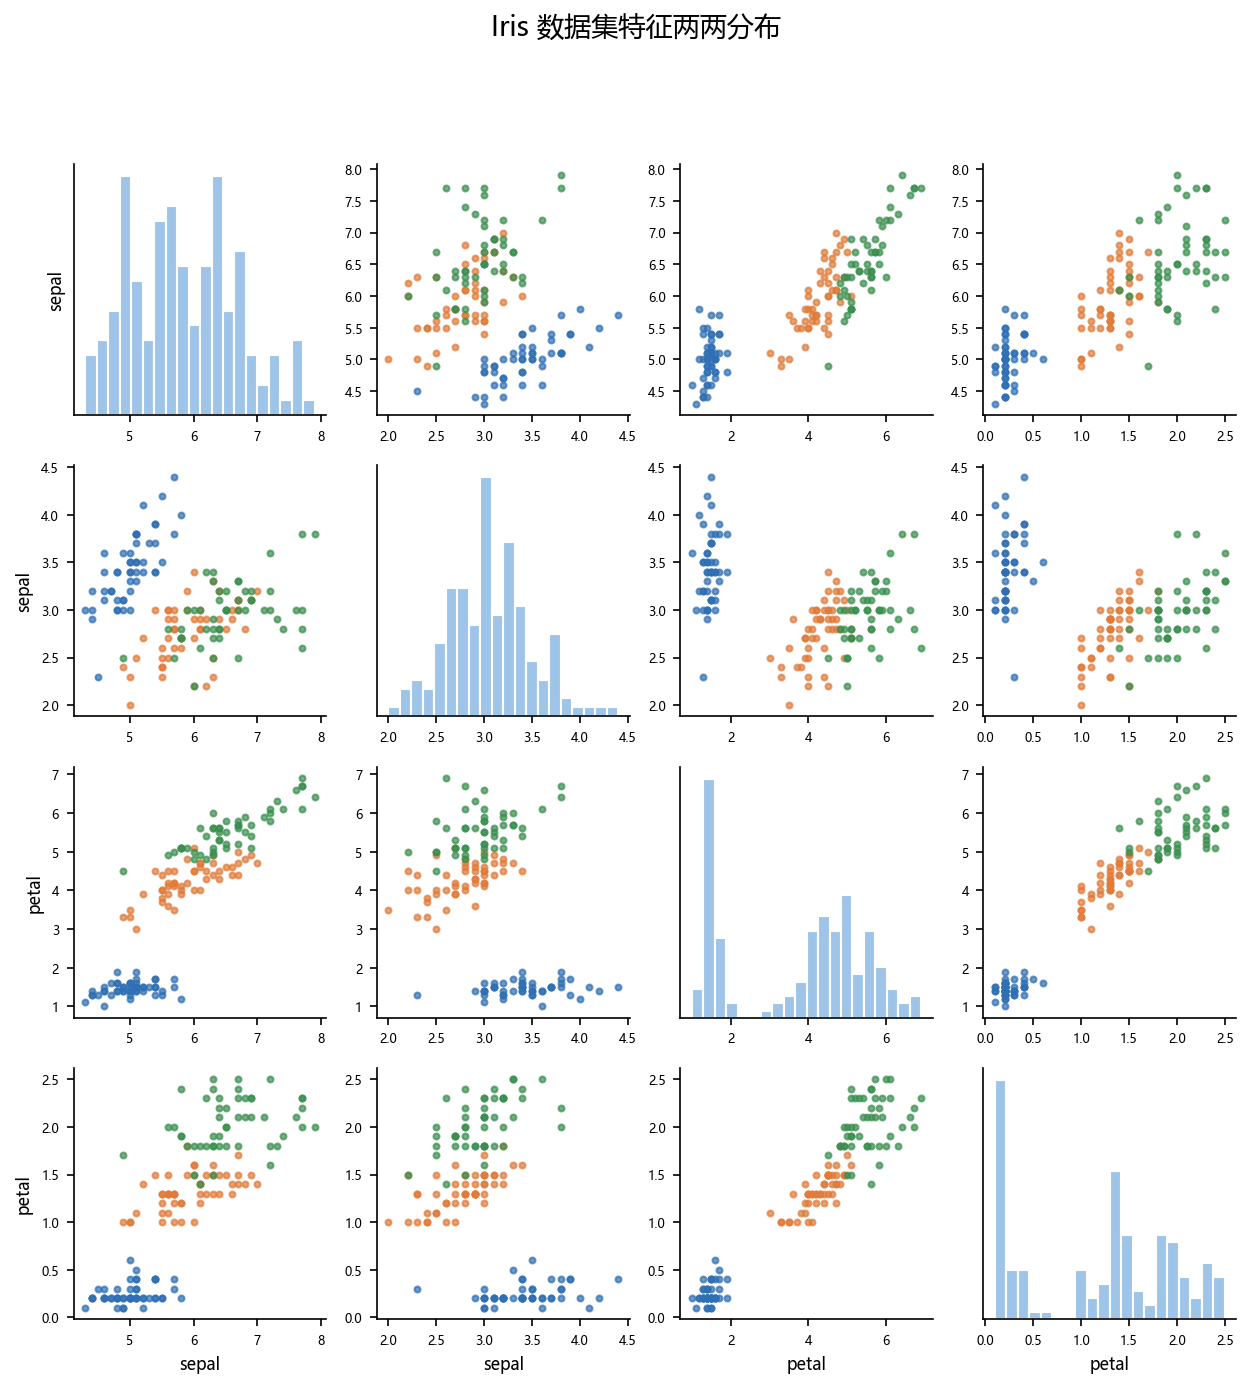
\includegraphics[keepaspectratio,alt={Iris 特征两两分布}]{figures/08-sklearn/iris_pairplot.png}}
\caption{Iris 特征两两分布}
\end{figure}

\paragraph{1.1
加载数据并切分}\label{ux52a0ux8f7dux6570ux636eux5e76ux5207ux5206}

\begin{Shaded}
\begin{Highlighting}[]
\ImportTok{import}\NormalTok{ numpy }\ImportTok{as}\NormalTok{ np}
\ImportTok{from}\NormalTok{ sklearn.datasets }\ImportTok{import}\NormalTok{ load\_iris}
\ImportTok{from}\NormalTok{ sklearn.model\_selection }\ImportTok{import}\NormalTok{ train\_test\_split}

\NormalTok{iris }\OperatorTok{=}\NormalTok{ load\_iris()}
\NormalTok{X, y }\OperatorTok{=}\NormalTok{ iris.data, iris.target}
\BuiltInTok{print}\NormalTok{(}\StringTok{"特征名:"}\NormalTok{, iris.feature\_names)}
\BuiltInTok{print}\NormalTok{(}\StringTok{"标签名:"}\NormalTok{, iris.target\_names)}
\BuiltInTok{print}\NormalTok{(}\StringTok{"数据形状:"}\NormalTok{, X.shape)}

\NormalTok{Xtr, Xte, ytr, yte }\OperatorTok{=}\NormalTok{ train\_test\_split(X, y, test\_size}\OperatorTok{=}\FloatTok{0.3}\NormalTok{, random\_state}\OperatorTok{=}\DecValTok{42}\NormalTok{, stratify}\OperatorTok{=}\NormalTok{y)}
\BuiltInTok{print}\NormalTok{(}\StringTok{"train/test:"}\NormalTok{, Xtr.shape, Xte.shape)}
\end{Highlighting}
\end{Shaded}

\begin{Shaded}
\begin{Highlighting}[]
\NormalTok{特征名: [\textquotesingle{}sepal length (cm)\textquotesingle{}, \textquotesingle{}sepal width (cm)\textquotesingle{}, \textquotesingle{}petal length (cm)\textquotesingle{}, \textquotesingle{}petal width (cm)\textquotesingle{}]}
\NormalTok{标签名: [\textquotesingle{}setosa\textquotesingle{} \textquotesingle{}versicolor\textquotesingle{} \textquotesingle{}virginica\textquotesingle{}]}
\NormalTok{数据形状: (150, 4)}
\NormalTok{train/test: (105, 4) (45, 4)}
\end{Highlighting}
\end{Shaded}

\paragraph{1.2
训练多个分类器并比较}\label{ux8badux7ec3ux591aux4e2aux5206ux7c7bux5668ux5e76ux6bd4ux8f83}

\begin{Shaded}
\begin{Highlighting}[]
\ImportTok{from}\NormalTok{ sklearn.neighbors }\ImportTok{import}\NormalTok{ KNeighborsClassifier}
\ImportTok{from}\NormalTok{ sklearn.linear\_model }\ImportTok{import}\NormalTok{ LogisticRegression}
\ImportTok{from}\NormalTok{ sklearn.tree }\ImportTok{import}\NormalTok{ DecisionTreeClassifier}
\ImportTok{from}\NormalTok{ sklearn.ensemble }\ImportTok{import}\NormalTok{ RandomForestClassifier}
\ImportTok{from}\NormalTok{ sklearn.metrics }\ImportTok{import}\NormalTok{ accuracy\_score}

\NormalTok{models }\OperatorTok{=}\NormalTok{ \{}
    \StringTok{"KNN(k=5)"}\NormalTok{: KNeighborsClassifier(n\_neighbors}\OperatorTok{=}\DecValTok{5}\NormalTok{),}
    \StringTok{"LogisticRegression"}\NormalTok{: LogisticRegression(max\_iter}\OperatorTok{=}\DecValTok{1000}\NormalTok{),}
    \StringTok{"DecisionTree"}\NormalTok{: DecisionTreeClassifier(random\_state}\OperatorTok{=}\DecValTok{42}\NormalTok{),}
    \StringTok{"RandomForest(100)"}\NormalTok{: RandomForestClassifier(n\_estimators}\OperatorTok{=}\DecValTok{100}\NormalTok{, random\_state}\OperatorTok{=}\DecValTok{42}\NormalTok{),}
\NormalTok{\}}
\ControlFlowTok{for}\NormalTok{ name, m }\KeywordTok{in}\NormalTok{ models.items():}
\NormalTok{    m.fit(Xtr, ytr)}
    \BuiltInTok{print}\NormalTok{(}\SpecialStringTok{f"}\SpecialCharTok{\{}\NormalTok{name}\SpecialCharTok{:22s\}}\SpecialStringTok{ acc = }\SpecialCharTok{\{}\NormalTok{accuracy\_score(yte, m.predict(Xte))}\SpecialCharTok{:.4f\}}\SpecialStringTok{"}\NormalTok{)}
\end{Highlighting}
\end{Shaded}

\begin{Shaded}
\begin{Highlighting}[]
\NormalTok{KNN(k=5)              acc = 0.9778}
\NormalTok{LogisticRegression    acc = 0.9333}
\NormalTok{DecisionTree          acc = 0.9333}
\NormalTok{RandomForest(100)     acc = 0.8889}
\end{Highlighting}
\end{Shaded}

\begin{quote}
不同模型在同一数据上表现不同，没有对任何数据集都最优的``万能模型''。随机森林在这份固定切分上反而略低，说明小样本下模型选择要看交叉验证与多次随机切分，而非一次
test 结果。
\end{quote}

\paragraph{1.3
混淆矩阵与分类报告}\label{ux6df7ux6dc6ux77e9ux9635ux4e0eux5206ux7c7bux62a5ux544a}

\begin{Shaded}
\begin{Highlighting}[]
\ImportTok{from}\NormalTok{ sklearn.metrics }\ImportTok{import}\NormalTok{ confusion\_matrix, classification\_report}

\NormalTok{rf }\OperatorTok{=}\NormalTok{ models[}\StringTok{"RandomForest(100)"}\NormalTok{]}
\BuiltInTok{print}\NormalTok{(confusion\_matrix(yte, rf.predict(Xte)))}
\BuiltInTok{print}\NormalTok{(classification\_report(yte, rf.predict(Xte), target\_names}\OperatorTok{=}\NormalTok{iris.target\_names))}
\end{Highlighting}
\end{Shaded}

\begin{Shaded}
\begin{Highlighting}[]
\NormalTok{[[15  0  0]}
\NormalTok{ [ 0 14  1]}
\NormalTok{ [ 0  4 11]]}
\NormalTok{              precision    recall  f1{-}score   support}

\NormalTok{      setosa       1.00      1.00      1.00        15}
\NormalTok{  versicolor       0.78      0.93      0.85        15}
\NormalTok{   virginica       0.92      0.73      0.81        15}

\NormalTok{    accuracy                           0.89        45}
\NormalTok{   macro avg       0.90      0.89      0.89        45}
\NormalTok{weighted avg       0.90      0.89      0.89        45}
\end{Highlighting}
\end{Shaded}

\begin{quote}
混淆矩阵第 i 行第 j 列表示``真实为 i、被判为
j''。\texttt{classification\_report} 给出每类的
precision、recall、f1。对不平衡数据，准确率会误导，要看 f1/recall。
\end{quote}

\paragraph{1.4 决策树可视化}\label{ux51b3ux7b56ux6811ux53efux89c6ux5316}

\begin{Shaded}
\begin{Highlighting}[]
\ImportTok{import}\NormalTok{ matplotlib.pyplot }\ImportTok{as}\NormalTok{ plt}
\NormalTok{plt.rcParams[}\StringTok{"font.sans{-}serif"}\NormalTok{] }\OperatorTok{=}\NormalTok{ [}\StringTok{"Microsoft YaHei"}\NormalTok{, }\StringTok{"SimHei"}\NormalTok{, }\StringTok{"DejaVu Sans"}\NormalTok{]}
\NormalTok{plt.rcParams[}\StringTok{"axes.unicode\_minus"}\NormalTok{] }\OperatorTok{=} \VariableTok{False}
\ImportTok{from}\NormalTok{ sklearn.tree }\ImportTok{import}\NormalTok{ plot\_tree}

\NormalTok{dt }\OperatorTok{=}\NormalTok{ DecisionTreeClassifier(max\_depth}\OperatorTok{=}\DecValTok{3}\NormalTok{, random\_state}\OperatorTok{=}\DecValTok{42}\NormalTok{).fit(Xtr, ytr)}
\NormalTok{fig, ax }\OperatorTok{=}\NormalTok{ plt.subplots(figsize}\OperatorTok{=}\NormalTok{(}\DecValTok{13}\NormalTok{, }\DecValTok{7}\NormalTok{))}
\NormalTok{plot\_tree(dt, feature\_names}\OperatorTok{=}\NormalTok{iris.feature\_names,}
\NormalTok{          class\_names}\OperatorTok{=}\BuiltInTok{list}\NormalTok{(iris.target\_names), filled}\OperatorTok{=}\VariableTok{True}\NormalTok{, rounded}\OperatorTok{=}\VariableTok{True}\NormalTok{, ax}\OperatorTok{=}\NormalTok{ax, fontsize}\OperatorTok{=}\DecValTok{8}\NormalTok{)}
\NormalTok{plt.title(}\StringTok{"Iris 决策树（max\_depth=3）"}\NormalTok{)}
\end{Highlighting}
\end{Shaded}

\begin{figure}
\centering
\pandocbounded{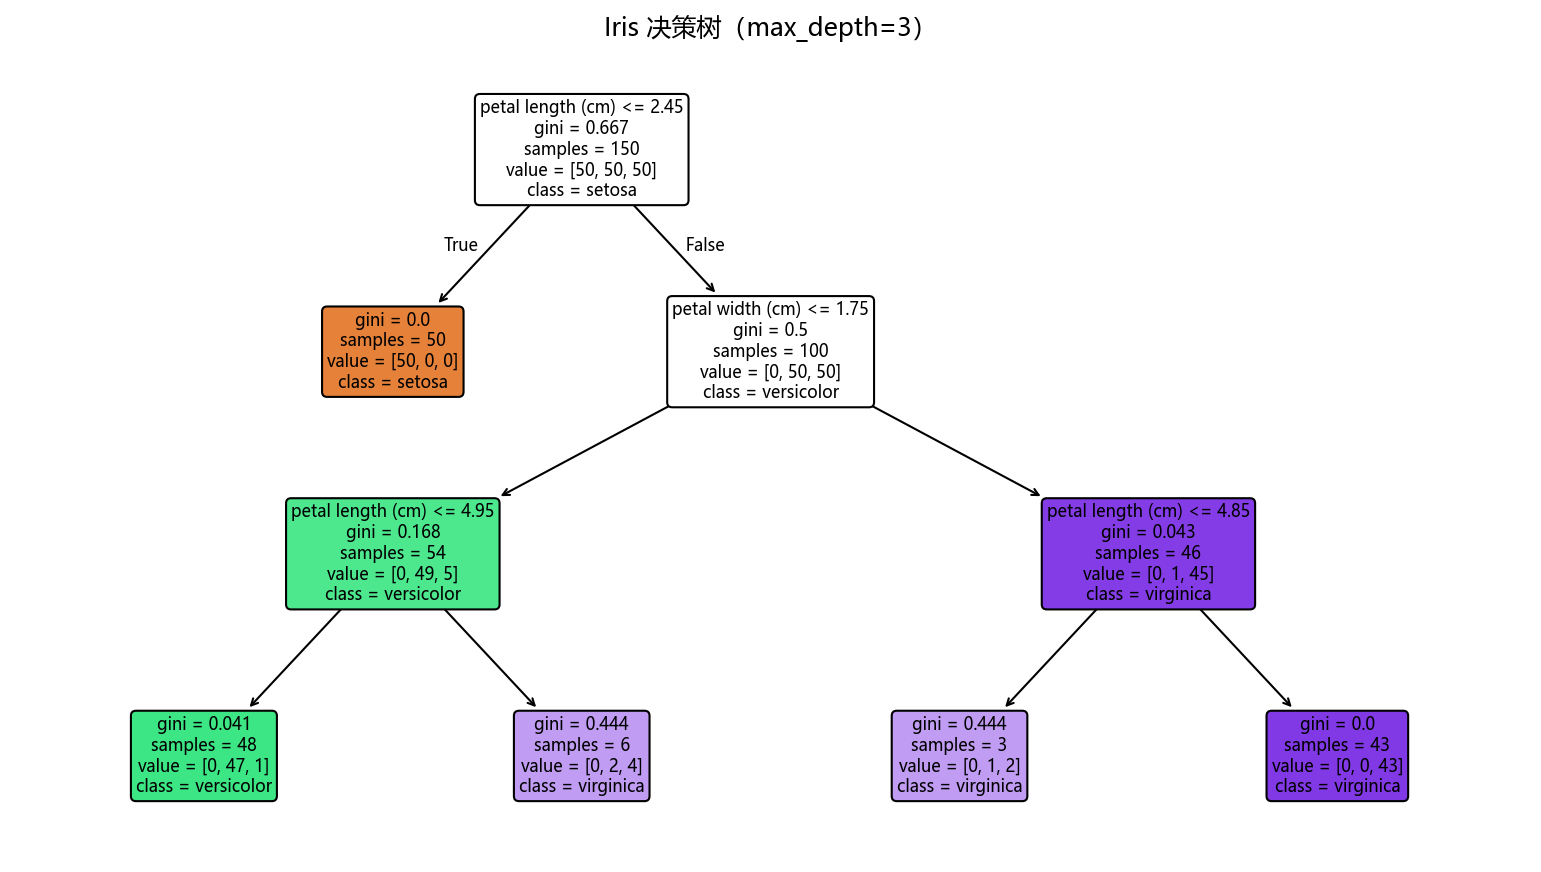
\includegraphics[keepaspectratio,alt={Iris 决策树}]{figures/08-sklearn/decision_tree_iris.png}}
\caption{Iris 决策树}
\end{figure}

\subsubsection{2. 二分类与
ROC-AUC：乳腺癌}\label{ux4e8cux5206ux7c7bux4e0e-roc-aucux4e73ux817aux764c}

乳腺癌数据集是二分类（良性/恶性）。逻辑回归对量纲敏感，因此用
\texttt{Pipeline} 先标准化再训练。

\begin{Shaded}
\begin{Highlighting}[]
\ImportTok{from}\NormalTok{ sklearn.datasets }\ImportTok{import}\NormalTok{ load\_breast\_cancer}
\ImportTok{from}\NormalTok{ sklearn.model\_selection }\ImportTok{import}\NormalTok{ train\_test\_split}
\ImportTok{from}\NormalTok{ sklearn.pipeline }\ImportTok{import}\NormalTok{ Pipeline}
\ImportTok{from}\NormalTok{ sklearn.preprocessing }\ImportTok{import}\NormalTok{ StandardScaler}
\ImportTok{from}\NormalTok{ sklearn.linear\_model }\ImportTok{import}\NormalTok{ LogisticRegression}
\ImportTok{from}\NormalTok{ sklearn.metrics }\ImportTok{import}\NormalTok{ accuracy\_score, roc\_auc\_score}

\NormalTok{bc }\OperatorTok{=}\NormalTok{ load\_breast\_cancer()}\OperatorTok{;}\NormalTok{ Xb, yb }\OperatorTok{=}\NormalTok{ bc.data, bc.target}
\NormalTok{Xtr, Xte, ytr, yte }\OperatorTok{=}\NormalTok{ train\_test\_split(Xb, yb, test\_size}\OperatorTok{=}\FloatTok{0.3}\NormalTok{, random\_state}\OperatorTok{=}\DecValTok{42}\NormalTok{, stratify}\OperatorTok{=}\NormalTok{yb)}

\NormalTok{pipe }\OperatorTok{=}\NormalTok{ Pipeline([(}\StringTok{"sc"}\NormalTok{, StandardScaler()), (}\StringTok{"clf"}\NormalTok{, LogisticRegression(max\_iter}\OperatorTok{=}\DecValTok{1000}\NormalTok{))])}
\NormalTok{pipe.fit(Xtr, ytr)}
\NormalTok{prob }\OperatorTok{=}\NormalTok{ pipe.predict\_proba(Xte)[:, }\DecValTok{1}\NormalTok{]}
\BuiltInTok{print}\NormalTok{(}\StringTok{"ROC{-}AUC:"}\NormalTok{, }\BuiltInTok{round}\NormalTok{(roc\_auc\_score(yte, prob), }\DecValTok{4}\NormalTok{))}
\BuiltInTok{print}\NormalTok{(}\StringTok{"准确率:"}\NormalTok{, }\BuiltInTok{round}\NormalTok{(accuracy\_score(yte, pipe.predict(Xte)), }\DecValTok{4}\NormalTok{))}
\end{Highlighting}
\end{Shaded}

\begin{Shaded}
\begin{Highlighting}[]
\NormalTok{ROC{-}AUC: 0.9981}
\NormalTok{准确率: 0.9883}
\end{Highlighting}
\end{Shaded}

\begin{quote}
\texttt{predict\_proba}
返回每个样本属于正类的概率；\texttt{roc\_auc\_score}
评估``排序能力''，比单纯准确率更能反映二分类模型质量。
\end{quote}

\textbf{缩放为什么关键}：SVC/KNN 对量纲很敏感。下图给出乳腺癌 5
折交叉验证，未标准化 vs 标准化的对比：

\begin{figure}
\centering
\pandocbounded{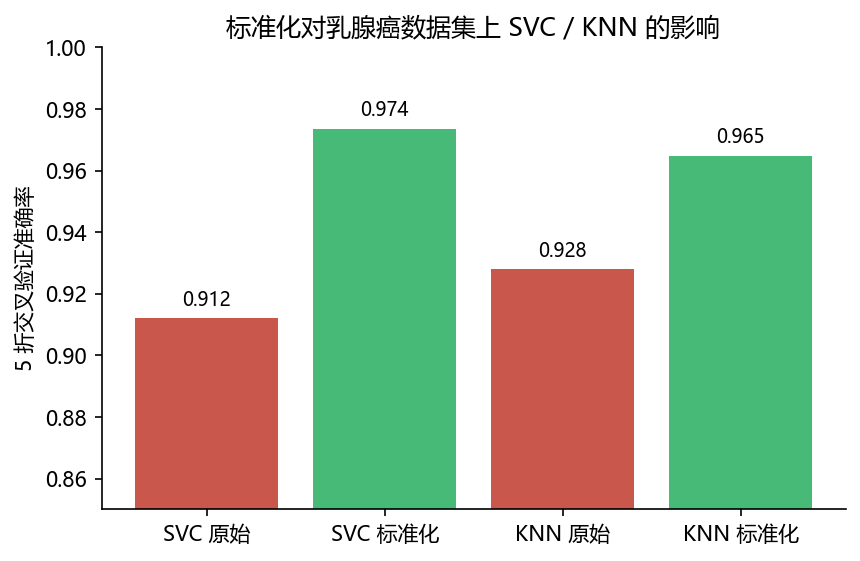
\includegraphics[keepaspectratio,alt={缩放影响}]{figures/08-sklearn/scaling_effect.png}}
\caption{缩放影响}
\end{figure}

\subsubsection{3. 回归：Diabetes
糖尿病}\label{ux56deux5f52diabetes-ux7cd6ux5c3fux75c5}

波士顿房价数据集（\texttt{load\_boston}）已在 sklearn 1.2
被移除，故本节改用内置的 \texttt{load\_diabetes}（442 个样本、10
个标准化后的特征）。

\begin{Shaded}
\begin{Highlighting}[]
\ImportTok{from}\NormalTok{ sklearn.datasets }\ImportTok{import}\NormalTok{ load\_diabetes}
\ImportTok{from}\NormalTok{ sklearn.model\_selection }\ImportTok{import}\NormalTok{ train\_test\_split}
\ImportTok{from}\NormalTok{ sklearn.linear\_model }\ImportTok{import}\NormalTok{ LinearRegression, Ridge, Lasso}
\ImportTok{from}\NormalTok{ sklearn.metrics }\ImportTok{import}\NormalTok{ mean\_squared\_error, mean\_absolute\_error, r2\_score}
\ImportTok{import}\NormalTok{ numpy }\ImportTok{as}\NormalTok{ np}

\NormalTok{d }\OperatorTok{=}\NormalTok{ load\_diabetes()}\OperatorTok{;}\NormalTok{ Xd, yd }\OperatorTok{=}\NormalTok{ d.data, d.target}
\NormalTok{Xtr, Xte, ytr, yte }\OperatorTok{=}\NormalTok{ train\_test\_split(Xd, yd, test\_size}\OperatorTok{=}\FloatTok{0.2}\NormalTok{, random\_state}\OperatorTok{=}\DecValTok{42}\NormalTok{)}

\ControlFlowTok{for}\NormalTok{ name, m }\KeywordTok{in}\NormalTok{ [(}\StringTok{"LinearRegression"}\NormalTok{, LinearRegression()),}
\NormalTok{                (}\StringTok{"Ridge(alpha=1)"}\NormalTok{, Ridge(alpha}\OperatorTok{=}\FloatTok{1.0}\NormalTok{)),}
\NormalTok{                (}\StringTok{"Lasso(alpha=0.1)"}\NormalTok{, Lasso(alpha}\OperatorTok{=}\FloatTok{0.1}\NormalTok{, max\_iter}\OperatorTok{=}\DecValTok{5000}\NormalTok{))]:}
\NormalTok{    m.fit(Xtr, ytr)}
\NormalTok{    yp }\OperatorTok{=}\NormalTok{ m.predict(Xte)}
    \BuiltInTok{print}\NormalTok{(}\SpecialStringTok{f"}\SpecialCharTok{\{}\NormalTok{name}\SpecialCharTok{:20s\}}\SpecialStringTok{ MSE=}\SpecialCharTok{\{}\NormalTok{mean\_squared\_error(yte, yp)}\SpecialCharTok{:.2f\}}\SpecialStringTok{  "}
          \SpecialStringTok{f"MAE=}\SpecialCharTok{\{}\NormalTok{mean\_absolute\_error(yte, yp)}\SpecialCharTok{:.2f\}}\SpecialStringTok{  R2=}\SpecialCharTok{\{}\NormalTok{r2\_score(yte, yp)}\SpecialCharTok{:.4f\}}\SpecialStringTok{"}\NormalTok{)}

\NormalTok{las }\OperatorTok{=}\NormalTok{ Lasso(alpha}\OperatorTok{=}\FloatTok{0.1}\NormalTok{, max\_iter}\OperatorTok{=}\DecValTok{5000}\NormalTok{).fit(Xtr, ytr)}
\BuiltInTok{print}\NormalTok{(}\StringTok{"Lasso 非零系数个数:"}\NormalTok{, np.count\_nonzero(las.coef\_))}
\BuiltInTok{print}\NormalTok{(}\StringTok{"特征名:"}\NormalTok{, d.feature\_names)}
\end{Highlighting}
\end{Shaded}

\begin{Shaded}
\begin{Highlighting}[]
\NormalTok{LinearRegression    MSE=2900.19  MAE=42.79  R2=0.4526}
\NormalTok{Ridge(alpha=1)      MSE=3077.42  MAE=46.14  R2=0.4192}
\NormalTok{Lasso(alpha=0.1)    MSE=2798.19  MAE=42.85  R2=0.4719}
\NormalTok{Lasso 非零系数个数: 7}
\NormalTok{特征名: [\textquotesingle{}age\textquotesingle{}, \textquotesingle{}sex\textquotesingle{}, \textquotesingle{}bmi\textquotesingle{}, \textquotesingle{}bp\textquotesingle{}, \textquotesingle{}s1\textquotesingle{}, \textquotesingle{}s2\textquotesingle{}, \textquotesingle{}s3\textquotesingle{}, \textquotesingle{}s4\textquotesingle{}, \textquotesingle{}s5\textquotesingle{}, \textquotesingle{}s6\textquotesingle{}]}
\end{Highlighting}
\end{Shaded}

\begin{quote}
回归指标速记：\texttt{MSE}/\texttt{MAE} 越小越好；\texttt{R2} 越接近 1
越好。这里 Lasso 用 L1 正则把部分系数压到 0，既得到不错 R²
又做了特征选择。
\end{quote}

\subsection{常见误区}\label{ux5e38ux89c1ux8befux533a-22}

\begin{enumerate}
\def\labelenumi{\arabic{enumi}.}
\tightlist
\item
  用 \texttt{r2\_score(y\_pred,\ y\_test)} 参数顺序写反 → 应为
  \texttt{r2\_score(y\_true,\ y\_pred)}；对分类问题更不该用 R²。
\item
  在 sklearn 里已经移除 \texttt{load\_boston}，再用会
  \texttt{ImportError}。
\item
  直接拿未缩放数据喂
  \texttt{SVC}/\texttt{KNN}/\texttt{LogisticRegression}，会导致收敛慢或精度差。
\item
  把 \texttt{predict\_proba} 的第一列当作正类概率 → 正类是第 1
  列（标签为 1 的类）。
\item
  在同一个数据集上反复``调参、看测试集''，相当于把测试集当训练信息用。
\end{enumerate}

\subsection{思考题}\label{ux601dux8003ux9898-22}

\begin{enumerate}
\def\labelenumi{\arabic{enumi}.}
\tightlist
\item
  为什么 KNN 对缩放特别敏感？树模型为什么相对不敏感？
\item
  \texttt{accuracy\_score} 与 \texttt{roc\_auc\_score}
  分别衡量什么？在类别不平衡时哪个更可靠？
\item
  一次 test 集准确率高，能说明模型泛化好吗？为什么还要交叉验证？
\end{enumerate}

\subsection{动手练习}\label{ux52a8ux624bux7ec3ux4e60-6}

\begin{enumerate}
\def\labelenumi{\arabic{enumi}.}
\tightlist
\item
  在 Iris 上把 \texttt{RandomForestClassifier(n\_estimators=100)} 与
  \texttt{KNeighborsClassifier} 做 5 折交叉验证比较。
\item
  用 \texttt{SVC} 分别在不缩放/缩放情况下做乳腺癌 5 折，记录结果（可对照
  \texttt{scaling\_effect.png}）。
\item
  在 Diabetes 上试 \texttt{Ridge(alpha)} 与 \texttt{Lasso(alpha)} 的不同
  \texttt{alpha} 值，画出``alpha-R²''曲线。
\end{enumerate}

\subsection{延伸阅读}\label{ux5ef6ux4f38ux9605ux8bfb-35}

\begin{itemize}
\tightlist
\item
  sklearn
  分类指标：https://scikit-learn.org/stable/modules/model\_evaluation.html\#classification-metrics
\item
  sklearn
  回归指标：https://scikit-learn.org/stable/modules/model\_evaluation.html\#regression-metrics
\item
  sklearn
  用户指南``选择正确的评估器''：https://scikit-learn.org/stable/modules/preprocessing.html
\end{itemize}

\section{03
无监督学习的案例}\label{ux65e0ux76d1ux7763ux5b66ux4e60ux7684ux6848ux4f8b}

\begin{quote}
本节讲``没有标签''的任务：\textbf{聚类}（KMeans、DBSCAN）与\textbf{降维}（PCA、LDA）。所有代码在
sklearn 1.6.1 下验证。
\end{quote}

\subsection{本节目标}\label{ux672cux8282ux76eeux6807-23}

\begin{enumerate}
\def\labelenumi{\arabic{enumi}.}
\tightlist
\item
  用 \texttt{KMeans} 对 \texttt{make\_blobs} 聚类，读出
  \texttt{inertia\_}、\texttt{cluster\_centers\_}、\texttt{silhouette\_score}。
\item
  用 \texttt{DBSCAN} 对 \texttt{make\_moons} 聚类，识别噪声（标签
  -1），并算 \texttt{adjusted\_rand\_score}。
\item
  用 \texttt{PCA} 降维并读出 \texttt{explained\_variance\_ratio\_}。
\item
  用 \texttt{LDA} 做有监督降维，理解它与 PCA 的差别。
\end{enumerate}

\subsection{先修}\label{ux5148ux4fee-23}

\begin{itemize}
\tightlist
\item
  01 节特征缩放、02 节分类/回归基础。
\item
  了解``距离''\,``方差''\,``协方差''等概念。
\end{itemize}

\subsection{官方文档 /
参考入口}\label{ux5b98ux65b9ux6587ux6863-ux53c2ux8003ux5165ux53e3-9}

\begin{itemize}
\tightlist
\item
  sklearn 聚类：https://scikit-learn.org/stable/modules/clustering.html
\item
  sklearn
  降维：https://scikit-learn.org/stable/modules/decomposition.html
\item
  sklearn
  聚类评估：https://scikit-learn.org/stable/modules/clustering.html\#clustering-performance-evaluation
\end{itemize}

\subsection{正文}\label{ux6b63ux6587-2}

\subsubsection{1. 聚类：KMeans}\label{ux805aux7c7bkmeans}

KMeans 把数据分成 K 个簇，使``簇内平方和''最小。它需要预先指定 K。

\begin{Shaded}
\begin{Highlighting}[]
\ImportTok{import}\NormalTok{ numpy }\ImportTok{as}\NormalTok{ np}
\ImportTok{from}\NormalTok{ sklearn.cluster }\ImportTok{import}\NormalTok{ KMeans}
\ImportTok{from}\NormalTok{ sklearn.datasets }\ImportTok{import}\NormalTok{ make\_blobs}
\ImportTok{from}\NormalTok{ sklearn.metrics }\ImportTok{import}\NormalTok{ silhouette\_score}

\NormalTok{X, \_ }\OperatorTok{=}\NormalTok{ make\_blobs(n\_samples}\OperatorTok{=}\DecValTok{300}\NormalTok{, centers}\OperatorTok{=}\DecValTok{4}\NormalTok{, cluster\_std}\OperatorTok{=}\FloatTok{0.60}\NormalTok{, random\_state}\OperatorTok{=}\DecValTok{0}\NormalTok{)}
\NormalTok{km }\OperatorTok{=}\NormalTok{ KMeans(n\_clusters}\OperatorTok{=}\DecValTok{4}\NormalTok{, random\_state}\OperatorTok{=}\DecValTok{0}\NormalTok{).fit(X)}
\NormalTok{labels }\OperatorTok{=}\NormalTok{ km.labels\_}
\BuiltInTok{print}\NormalTok{(}\StringTok{"inertia:"}\NormalTok{, }\BuiltInTok{round}\NormalTok{(km.inertia\_, }\DecValTok{4}\NormalTok{))}
\BuiltInTok{print}\NormalTok{(}\StringTok{"聚类中心形状:"}\NormalTok{, km.cluster\_centers\_.shape)}
\BuiltInTok{print}\NormalTok{(}\StringTok{"轮廓系数:"}\NormalTok{, }\BuiltInTok{round}\NormalTok{(silhouette\_score(X, labels), }\DecValTok{4}\NormalTok{))}
\end{Highlighting}
\end{Shaded}

\begin{Shaded}
\begin{Highlighting}[]
\NormalTok{inertia: 212.006}
\NormalTok{聚类中心形状: (4, 2)}
\NormalTok{轮廓系数: 0.682}
\end{Highlighting}
\end{Shaded}

\begin{quote}
\texttt{inertia\_} 是簇内平方和，越小越好；\texttt{silhouette\_score} 在
{[}-1,1{]} 之间，越接近 1 表示簇内紧凑、簇间分离越好。
\end{quote}

\subsubsection{2. 聚类：DBSCAN}\label{ux805aux7c7bdbscan}

DBSCAN 按密度自动发现簇，能处理任意形状，并能把不属于任何簇的点标为
\textbf{-1（噪声）}。

\begin{Shaded}
\begin{Highlighting}[]
\ImportTok{from}\NormalTok{ sklearn.cluster }\ImportTok{import}\NormalTok{ DBSCAN}
\ImportTok{from}\NormalTok{ sklearn.datasets }\ImportTok{import}\NormalTok{ make\_moons}
\ImportTok{from}\NormalTok{ sklearn.metrics }\ImportTok{import}\NormalTok{ adjusted\_rand\_score}

\NormalTok{Xm, ym }\OperatorTok{=}\NormalTok{ make\_moons(n\_samples}\OperatorTok{=}\DecValTok{300}\NormalTok{, noise}\OperatorTok{=}\FloatTok{0.1}\NormalTok{, random\_state}\OperatorTok{=}\DecValTok{42}\NormalTok{)}
\NormalTok{db }\OperatorTok{=}\NormalTok{ DBSCAN(eps}\OperatorTok{=}\FloatTok{0.2}\NormalTok{, min\_samples}\OperatorTok{=}\DecValTok{5}\NormalTok{).fit(Xm)}
\NormalTok{labels }\OperatorTok{=}\NormalTok{ db.labels\_}
\BuiltInTok{print}\NormalTok{(}\StringTok{"簇数:"}\NormalTok{, }\BuiltInTok{len}\NormalTok{(}\BuiltInTok{set}\NormalTok{(labels)) }\OperatorTok{{-}}\NormalTok{ (}\DecValTok{1} \ControlFlowTok{if} \OperatorTok{{-}}\DecValTok{1} \KeywordTok{in}\NormalTok{ labels }\ControlFlowTok{else} \DecValTok{0}\NormalTok{))}
\BuiltInTok{print}\NormalTok{(}\StringTok{"噪声比例:"}\NormalTok{, }\BuiltInTok{round}\NormalTok{(np.mean(labels }\OperatorTok{==} \OperatorTok{{-}}\DecValTok{1}\NormalTok{), }\DecValTok{4}\NormalTok{))}
\BuiltInTok{print}\NormalTok{(}\StringTok{"簇大小:"}\NormalTok{, np.bincount(labels))}
\BuiltInTok{print}\NormalTok{(}\StringTok{"与真实标签 ARI:"}\NormalTok{, }\BuiltInTok{round}\NormalTok{(adjusted\_rand\_score(ym, labels), }\DecValTok{4}\NormalTok{))}
\end{Highlighting}
\end{Shaded}

\begin{Shaded}
\begin{Highlighting}[]
\NormalTok{簇数: 2}
\NormalTok{噪声比例: 0.0}
\NormalTok{簇大小: [150 150]}
\NormalTok{与真实标签 ARI: 1.0}
\end{Highlighting}
\end{Shaded}

\begin{quote}
\texttt{adjusted\_rand\_score}（ARI）在 {[}0,1{]}（随机约 0、完全一致为
1）。这里 DBSCAN 完美分出两个月牙形簇，ARI=1.0。
\end{quote}

\textbf{KMeans 与 DBSCAN 的对比}：KMeans
假设凸形、球形簇，对``弯月''类数据效果差；DBSCAN
依据密度，可发现任意形状并识别噪声。

\begin{figure}
\centering
\pandocbounded{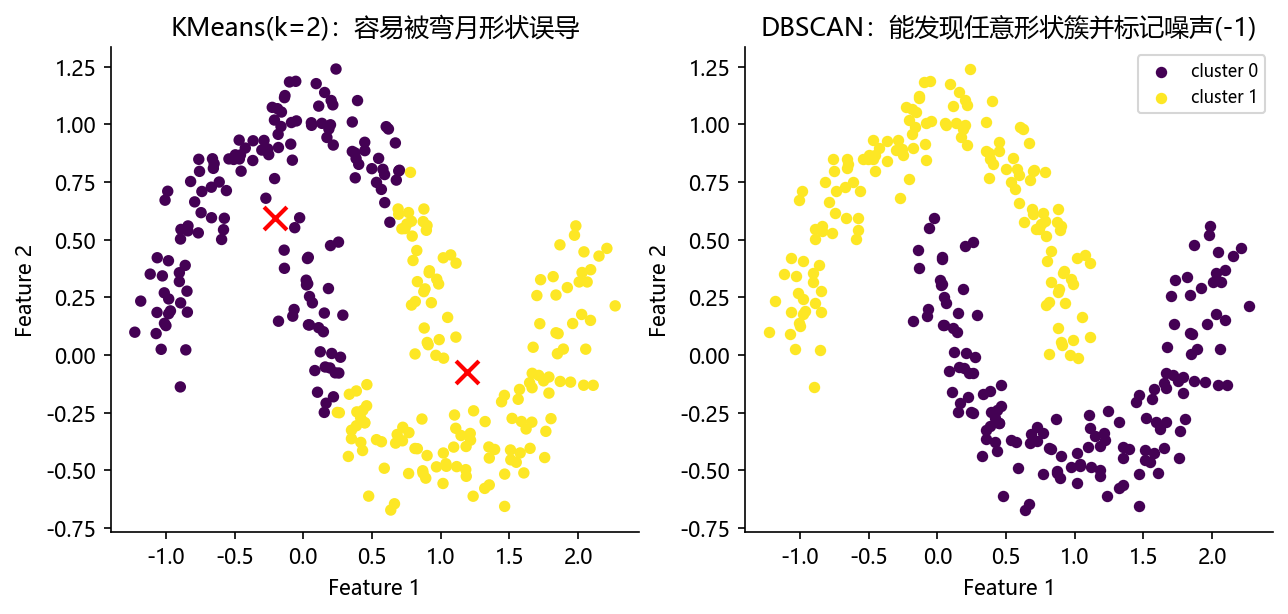
\includegraphics[keepaspectratio,alt={KMeans vs DBSCAN}]{figures/08-sklearn/dbscan_kmeans_moons.png}}
\caption{KMeans vs DBSCAN}
\end{figure}

\subsubsection{3.
降维：PCA（无监督）}\label{ux964dux7ef4pcaux65e0ux76d1ux7763}

PCA 找``方差最大的方向''，把高维映射到低维，且不需要标签。

\begin{Shaded}
\begin{Highlighting}[]
\ImportTok{from}\NormalTok{ sklearn.datasets }\ImportTok{import}\NormalTok{ load\_iris}
\ImportTok{from}\NormalTok{ sklearn.decomposition }\ImportTok{import}\NormalTok{ PCA}

\NormalTok{iris }\OperatorTok{=}\NormalTok{ load\_iris()}\OperatorTok{;}\NormalTok{ X, y }\OperatorTok{=}\NormalTok{ iris.data, iris.target}
\NormalTok{pca }\OperatorTok{=}\NormalTok{ PCA(n\_components}\OperatorTok{=}\DecValTok{2}\NormalTok{)}
\NormalTok{Xp }\OperatorTok{=}\NormalTok{ pca.fit\_transform(X)}
\BuiltInTok{print}\NormalTok{(}\StringTok{"各主成分解释方差比:"}\NormalTok{, np.}\BuiltInTok{round}\NormalTok{(pca.explained\_variance\_ratio\_, }\DecValTok{4}\NormalTok{))}
\BuiltInTok{print}\NormalTok{(}\StringTok{"累计解释方差:"}\NormalTok{, np.}\BuiltInTok{round}\NormalTok{(np.cumsum(pca.explained\_variance\_ratio\_), }\DecValTok{4}\NormalTok{))}
\end{Highlighting}
\end{Shaded}

\begin{Shaded}
\begin{Highlighting}[]
\NormalTok{各主成分解释方差比: [0.9246 0.0531]}
\NormalTok{累计解释方差: [0.9246 0.9777]}
\end{Highlighting}
\end{Shaded}

\begin{quote}
前 2 个主成分已保留约 97.77\% 方差，说明 Iris 降到 2
维几乎不丢信息，适合可视化。
\end{quote}

\subsubsection{4.
降维：LDA（有监督）}\label{ux964dux7ef4ldaux6709ux76d1ux7763}

LDA
在已知类别的情况下，找``类间方差最大、类内方差最小''的投影方向。因此需要同时给出
\texttt{X} 与 \texttt{y}。

\begin{Shaded}
\begin{Highlighting}[]
\ImportTok{from}\NormalTok{ sklearn.discriminant\_analysis }\ImportTok{import}\NormalTok{ LinearDiscriminantAnalysis }\ImportTok{as}\NormalTok{ LDA}

\NormalTok{lda }\OperatorTok{=}\NormalTok{ LDA(n\_components}\OperatorTok{=}\DecValTok{2}\NormalTok{)}
\NormalTok{Xl }\OperatorTok{=}\NormalTok{ lda.fit\_transform(X, y)}
\BuiltInTok{print}\NormalTok{(}\StringTok{"LDA 各成分解释方差比:"}\NormalTok{, np.}\BuiltInTok{round}\NormalTok{(lda.explained\_variance\_ratio\_, }\DecValTok{4}\NormalTok{))}
\end{Highlighting}
\end{Shaded}

\begin{Shaded}
\begin{Highlighting}[]
\NormalTok{LDA 各成分解释方差比: [0.9912 0.0088]}
\end{Highlighting}
\end{Shaded}

\begin{quote}
对比：PCA 完全不看类别，LDA
用类别信息，因而投影对分类更有帮助。两者都适用于 Iris 降到 2
维，但语义不同。
\end{quote}

\subsection{常见误区}\label{ux5e38ux89c1ux8befux533a-23}

\begin{enumerate}
\def\labelenumi{\arabic{enumi}.}
\tightlist
\item
  KMeans 必须预设 \texttt{n\_clusters}，且对初始中心敏感（用
  \texttt{random\_state} 固定，或用 \texttt{k-means++}）。
\item
  以为``降维能提升所有模型精度''------降维会丢失信息，有时反而更差。
\item
  把 PCA 与 LDA 混为一谈（前者无监督、后者有监督）。
\item
  对 \texttt{make\_moons} 用 KMeans 期望得到月牙形簇------通常失败。
\item
  \texttt{DBSCAN} 的 \texttt{eps}、\texttt{min\_samples}
  必须按数据量纲调，不能``一个参数跑天下''。
\end{enumerate}

\subsection{思考题}\label{ux601dux8003ux9898-23}

\begin{enumerate}
\def\labelenumi{\arabic{enumi}.}
\tightlist
\item
  为什么 KMeans 需要先缩放？PCA 呢？
\item
  DBSCAN 的 \texttt{eps} 太小/太大会分别出现什么现象？
\item
  用什么指标判断``该保留多少个主成分''？（累计解释方差、碎石图等）
\item
  ARI 与 \texttt{silhouette\_score} 的适用场景有何不同？
\end{enumerate}

\subsection{动手练习}\label{ux52a8ux624bux7ec3ux4e60-7}

\begin{enumerate}
\def\labelenumi{\arabic{enumi}.}
\tightlist
\item
  对 \texttt{make\_blobs} 用 \texttt{KMeans(k=2..6)}
  画出``k-轮廓系数''曲线，找最佳 k。
\item
  调整 \texttt{DBSCAN} 的
  \texttt{eps}（0.1/0.2/0.5），观察簇数与噪声比例变化。
\item
  对 Wine 数据（13 维）用 PCA 降到 2 维并散点着色，给出累计解释方差。
\end{enumerate}

\subsection{延伸阅读}\label{ux5ef6ux4f38ux9605ux8bfb-36}

\begin{itemize}
\tightlist
\item
  sklearn
  聚类用户指南：https://scikit-learn.org/stable/modules/clustering.html
\item
  sklearn
  降维用户指南：https://scikit-learn.org/stable/modules/decomposition.html
\item
  sklearn
  聚类评估：https://scikit-learn.org/stable/modules/clustering.html\#clustering-performance-evaluation
\end{itemize}

\section{04 综合案例：Wine 数据端到端（预处理 → 分类 → 聚类 →
降维）}\label{ux7efcux5408ux6848ux4f8bwine-ux6570ux636eux7aefux5230ux7aefux9884ux5904ux7406-ux5206ux7c7b-ux805aux7c7b-ux964dux7ef4}

\begin{quote}
本章新增综合案例，把 01--03 的知识串成一条完整流水线：\textbf{特征缩放 →
分类 → 特征重要性 → 聚类 → 降维 → 可视化}。所有代码在 sklearn 1.6.1
下验证；配图由 \texttt{build/make\_chap8\_figures.py} 生成。
\end{quote}

\subsection{案例背景}\label{ux6848ux4f8bux80ccux666f-3}

Wine（红酒）数据集有 178 个样本、13
个数值特征（酒精、苹果酸、灰分、总酚、黄酮等），标签为 3
个品种（\texttt{class\_0/1/2}）。这是一个``数值特征多、量纲不同、类别有结构''的典型数据，非常适合练习本章全部知识。

\subsection{第 1
步：加载数据并观察}\label{ux7b2c-1-ux6b65ux52a0ux8f7dux6570ux636eux5e76ux89c2ux5bdf}

\begin{Shaded}
\begin{Highlighting}[]
\ImportTok{import}\NormalTok{ numpy }\ImportTok{as}\NormalTok{ np}
\ImportTok{from}\NormalTok{ sklearn.datasets }\ImportTok{import}\NormalTok{ load\_wine}

\NormalTok{wine }\OperatorTok{=}\NormalTok{ load\_wine()}
\NormalTok{X, y }\OperatorTok{=}\NormalTok{ wine.data, wine.target}
\BuiltInTok{print}\NormalTok{(}\StringTok{"特征名:"}\NormalTok{, wine.feature\_names)}
\BuiltInTok{print}\NormalTok{(}\StringTok{"数据形状:"}\NormalTok{, X.shape, }\StringTok{"类别:"}\NormalTok{, np.unique(y))}
\end{Highlighting}
\end{Shaded}

\begin{Shaded}
\begin{Highlighting}[]
\NormalTok{特征名: [\textquotesingle{}alcohol\textquotesingle{}, \textquotesingle{}malic\_acid\textquotesingle{}, \textquotesingle{}ash\textquotesingle{}, \textquotesingle{}alcalinity\_of\_ash\textquotesingle{}, \textquotesingle{}magnesium\textquotesingle{}, \textquotesingle{}total\_phenols\textquotesingle{}, \textquotesingle{}flavanoids\textquotesingle{}, \textquotesingle{}nonflavanoid\_phenols\textquotesingle{}, \textquotesingle{}proanthocyanins\textquotesingle{}, \textquotesingle{}color\_intensity\textquotesingle{}, \textquotesingle{}hue\textquotesingle{}, \textquotesingle{}od280/od315\_of\_diluted\_wines\textquotesingle{}, \textquotesingle{}proline\textquotesingle{}]}
\NormalTok{数据形状: (178, 13) 类别: [0 1 2]}
\end{Highlighting}
\end{Shaded}

\subsection{第 2 步：缩放 + 分类（用 Pipeline
防泄漏）}\label{ux7b2c-2-ux6b65ux7f29ux653e-ux5206ux7c7bux7528-pipeline-ux9632ux6cc4ux6f0f}

把``标准化''与``分类器''放进 \texttt{Pipeline}，这样
\texttt{cross\_val\_score}
每次都在训练折上拟合缩放器，绝不用测试折的信息。

\begin{Shaded}
\begin{Highlighting}[]
\ImportTok{from}\NormalTok{ sklearn.model\_selection }\ImportTok{import}\NormalTok{ train\_test\_split, cross\_val\_score}
\ImportTok{from}\NormalTok{ sklearn.preprocessing }\ImportTok{import}\NormalTok{ StandardScaler}
\ImportTok{from}\NormalTok{ sklearn.pipeline }\ImportTok{import}\NormalTok{ Pipeline}
\ImportTok{from}\NormalTok{ sklearn.linear\_model }\ImportTok{import}\NormalTok{ LogisticRegression}
\ImportTok{from}\NormalTok{ sklearn.ensemble }\ImportTok{import}\NormalTok{ RandomForestClassifier}
\ImportTok{from}\NormalTok{ sklearn.metrics }\ImportTok{import}\NormalTok{ accuracy\_score}

\NormalTok{Xtr, Xte, ytr, yte }\OperatorTok{=}\NormalTok{ train\_test\_split(X, y, test\_size}\OperatorTok{=}\FloatTok{0.3}\NormalTok{, random\_state}\OperatorTok{=}\DecValTok{42}\NormalTok{, stratify}\OperatorTok{=}\NormalTok{y)}
\BuiltInTok{print}\NormalTok{(}\StringTok{"train:"}\NormalTok{, Xtr.shape, }\StringTok{"test:"}\NormalTok{, Xte.shape)}

\NormalTok{lr\_pipe }\OperatorTok{=}\NormalTok{ Pipeline([(}\StringTok{"sc"}\NormalTok{, StandardScaler()), (}\StringTok{"clf"}\NormalTok{, LogisticRegression(max\_iter}\OperatorTok{=}\DecValTok{1000}\NormalTok{))])}
\NormalTok{rf\_pipe }\OperatorTok{=}\NormalTok{ Pipeline([(}\StringTok{"sc"}\NormalTok{, StandardScaler()), (}\StringTok{"clf"}\NormalTok{, RandomForestClassifier(n\_estimators}\OperatorTok{=}\DecValTok{100}\NormalTok{, random\_state}\OperatorTok{=}\DecValTok{42}\NormalTok{))])}

\NormalTok{lr\_pipe.fit(Xtr, ytr)}
\NormalTok{rf\_pipe.fit(Xtr, ytr)}
\BuiltInTok{print}\NormalTok{(}\StringTok{"LogisticRegression test acc:"}\NormalTok{, }\BuiltInTok{round}\NormalTok{(accuracy\_score(yte, lr\_pipe.predict(Xte)), }\DecValTok{4}\NormalTok{))}
\BuiltInTok{print}\NormalTok{(}\StringTok{"RandomForest      test acc:"}\NormalTok{, }\BuiltInTok{round}\NormalTok{(accuracy\_score(yte, rf\_pipe.predict(Xte)), }\DecValTok{4}\NormalTok{))}
\BuiltInTok{print}\NormalTok{(}\StringTok{"LogisticRegression 5 折均值:"}\NormalTok{, }\BuiltInTok{round}\NormalTok{(cross\_val\_score(lr\_pipe, X, y, cv}\OperatorTok{=}\DecValTok{5}\NormalTok{).mean(), }\DecValTok{4}\NormalTok{))}
\BuiltInTok{print}\NormalTok{(}\StringTok{"RandomForest      5 折均值:"}\NormalTok{, }\BuiltInTok{round}\NormalTok{(cross\_val\_score(rf\_pipe, X, y, cv}\OperatorTok{=}\DecValTok{5}\NormalTok{).mean(), }\DecValTok{4}\NormalTok{))}
\end{Highlighting}
\end{Shaded}

\begin{Shaded}
\begin{Highlighting}[]
\NormalTok{train: (124, 13) test: (54, 13)}
\NormalTok{LogisticRegression test acc: 0.9815}
\NormalTok{RandomForest      test acc: 1.0}
\NormalTok{LogisticRegression 5 折均值: 0.9832}
\NormalTok{RandomForest      5 折均值: 0.9778}
\end{Highlighting}
\end{Shaded}

\begin{quote}
真实项目里，一组固定的 test
集被反复调参会导致``测试集过拟合''；所以更稳的是看 5 折平均（这里
LogisticRegression 与 RandomForest 均约 0.98）。
\end{quote}

\subsection{第 3
步：特征重要性（RandomForest）}\label{ux7b2c-3-ux6b65ux7279ux5f81ux91cdux8981ux6027randomforest}

用随机森林的 \texttt{feature\_importances\_} 看哪些特征更重要。

\begin{Shaded}
\begin{Highlighting}[]
\ImportTok{from}\NormalTok{ sklearn.preprocessing }\ImportTok{import}\NormalTok{ StandardScaler}
\ImportTok{from}\NormalTok{ sklearn.ensemble }\ImportTok{import}\NormalTok{ RandomForestClassifier}

\NormalTok{Xs }\OperatorTok{=}\NormalTok{ StandardScaler().fit\_transform(X)}
\NormalTok{rf }\OperatorTok{=}\NormalTok{ RandomForestClassifier(n\_estimators}\OperatorTok{=}\DecValTok{100}\NormalTok{, random\_state}\OperatorTok{=}\DecValTok{42}\NormalTok{).fit(Xs, y)}
\NormalTok{imp }\OperatorTok{=}\NormalTok{ rf.feature\_importances\_}
\NormalTok{order }\OperatorTok{=}\NormalTok{ np.argsort(imp)[::}\OperatorTok{{-}}\DecValTok{1}\NormalTok{]}
\ControlFlowTok{for}\NormalTok{ i }\KeywordTok{in}\NormalTok{ order[:}\DecValTok{6}\NormalTok{]:}
    \BuiltInTok{print}\NormalTok{(}\SpecialStringTok{f"}\SpecialCharTok{\{}\NormalTok{wine}\SpecialCharTok{.}\NormalTok{feature\_names[i]}\SpecialCharTok{:30s\}}\SpecialStringTok{ }\SpecialCharTok{\{}\NormalTok{imp[i]}\SpecialCharTok{:.4f\}}\SpecialStringTok{"}\NormalTok{)}
\end{Highlighting}
\end{Shaded}

\begin{Shaded}
\begin{Highlighting}[]
\NormalTok{flavanoids                     0.1945}
\NormalTok{color\_intensity                0.1730}
\NormalTok{alcohol                        0.1416}
\NormalTok{proline                        0.1370}
\NormalTok{od280/od315\_of\_diluted\_wines   0.1118}
\NormalTok{hue                            0.0769}
\end{Highlighting}
\end{Shaded}

\begin{figure}
\centering
\pandocbounded{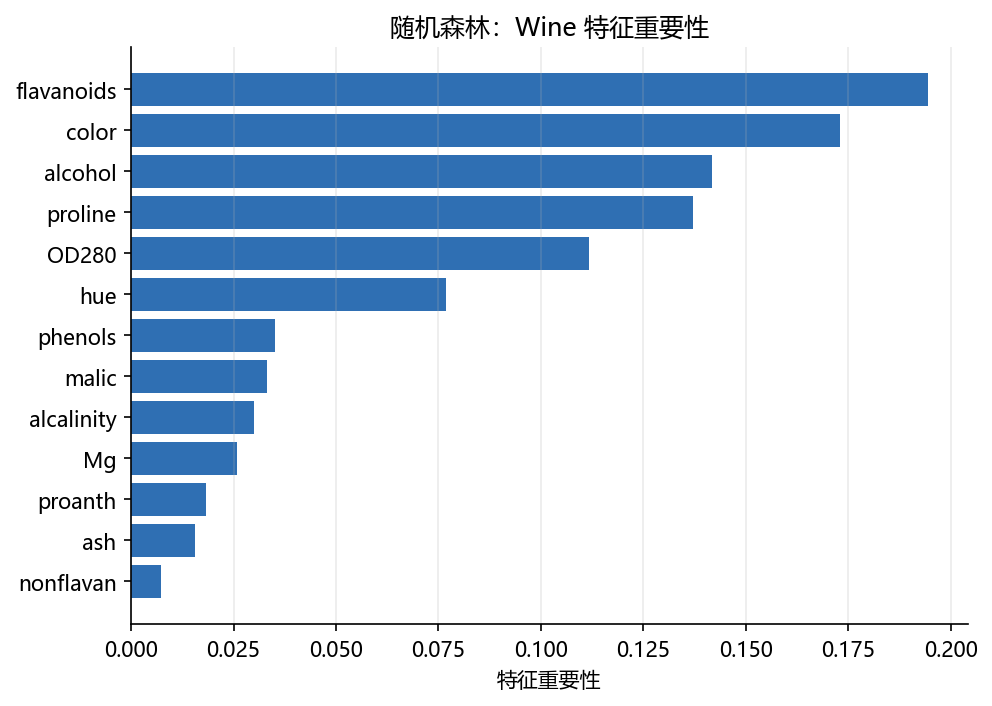
\includegraphics[keepaspectratio,alt={Wine 特征重要性}]{figures/08-sklearn/wine_feature_importance.png}}
\caption{Wine 特征重要性}
\end{figure}

\begin{quote}
黄酮（flavanoids）、颜色强度（color\_intensity）、酒精含量（alcohol）、脯氨酸（proline）等对品种区分贡献最大。这有助于我们``读懂''模型而不仅是得到一个分数。
\end{quote}

\subsection{第 4
步：无监督聚类（KMeans）}\label{ux7b2c-4-ux6b65ux65e0ux76d1ux7763ux805aux7c7bkmeans}

把``没有标签''的思路也用上：对标准化后的 Wine 做
KMeans，看能否大致还原真实品种。

\begin{Shaded}
\begin{Highlighting}[]
\ImportTok{from}\NormalTok{ sklearn.cluster }\ImportTok{import}\NormalTok{ KMeans}
\ImportTok{from}\NormalTok{ sklearn.metrics }\ImportTok{import}\NormalTok{ adjusted\_rand\_score, silhouette\_score}

\NormalTok{km }\OperatorTok{=}\NormalTok{ KMeans(n\_clusters}\OperatorTok{=}\DecValTok{3}\NormalTok{, random\_state}\OperatorTok{=}\DecValTok{42}\NormalTok{).fit(Xs)}
\BuiltInTok{print}\NormalTok{(}\StringTok{"轮廓系数:"}\NormalTok{, }\BuiltInTok{round}\NormalTok{(silhouette\_score(Xs, km.labels\_), }\DecValTok{4}\NormalTok{))}
\BuiltInTok{print}\NormalTok{(}\StringTok{"ARI vs 真实标签:"}\NormalTok{, }\BuiltInTok{round}\NormalTok{(adjusted\_rand\_score(y, km.labels\_), }\DecValTok{4}\NormalTok{))}
\BuiltInTok{print}\NormalTok{(}\StringTok{"各簇大小:"}\NormalTok{, np.bincount(km.labels\_))}
\end{Highlighting}
\end{Shaded}

\begin{Shaded}
\begin{Highlighting}[]
\NormalTok{轮廓系数: 0.2849}
\NormalTok{ARI vs 真实标签: 0.8975}
\NormalTok{各簇大小: [65 51 62]}
\end{Highlighting}
\end{Shaded}

\begin{quote}
\texttt{adjusted\_rand\_score=0.8975}
表示无监督聚类与真实品种高度一致（1 为完全一致），说明 Wine
数据确有明显的类结构。
\end{quote}

\subsection{第 5 步：PCA
降维并可视化}\label{ux7b2c-5-ux6b65pca-ux964dux7ef4ux5e76ux53efux89c6ux5316}

用 PCA 把 13 维压到 2 维，分别按真实类别与 KMeans 簇着色：

\begin{Shaded}
\begin{Highlighting}[]
\ImportTok{import}\NormalTok{ matplotlib.pyplot }\ImportTok{as}\NormalTok{ plt}
\NormalTok{plt.rcParams[}\StringTok{"font.sans{-}serif"}\NormalTok{] }\OperatorTok{=}\NormalTok{ [}\StringTok{"Microsoft YaHei"}\NormalTok{, }\StringTok{"SimHei"}\NormalTok{, }\StringTok{"DejaVu Sans"}\NormalTok{]}
\NormalTok{plt.rcParams[}\StringTok{"axes.unicode\_minus"}\NormalTok{] }\OperatorTok{=} \VariableTok{False}
\ImportTok{from}\NormalTok{ sklearn.decomposition }\ImportTok{import}\NormalTok{ PCA}

\NormalTok{pca }\OperatorTok{=}\NormalTok{ PCA(n\_components}\OperatorTok{=}\DecValTok{2}\NormalTok{)}
\NormalTok{Xp }\OperatorTok{=}\NormalTok{ pca.fit\_transform(Xs)}
\BuiltInTok{print}\NormalTok{(}\StringTok{"前两个主成分解释方差:"}\NormalTok{, np.}\BuiltInTok{round}\NormalTok{(pca.explained\_variance\_ratio\_, }\DecValTok{4}\NormalTok{))}
\BuiltInTok{print}\NormalTok{(}\StringTok{"累计解释方差:"}\NormalTok{, np.}\BuiltInTok{round}\NormalTok{(np.cumsum(pca.explained\_variance\_ratio\_), }\DecValTok{4}\NormalTok{))}

\NormalTok{fig, axes }\OperatorTok{=}\NormalTok{ plt.subplots(}\DecValTok{1}\NormalTok{, }\DecValTok{2}\NormalTok{, figsize}\OperatorTok{=}\NormalTok{(}\DecValTok{10}\NormalTok{, }\DecValTok{4}\NormalTok{))}
\NormalTok{axes[}\DecValTok{0}\NormalTok{].scatter(Xp[:, }\DecValTok{0}\NormalTok{], Xp[:, }\DecValTok{1}\NormalTok{], c}\OperatorTok{=}\NormalTok{y, cmap}\OperatorTok{=}\StringTok{"viridis"}\NormalTok{, s}\OperatorTok{=}\DecValTok{22}\NormalTok{)}
\NormalTok{axes[}\DecValTok{0}\NormalTok{].set\_title(}\StringTok{"PCA 按真实类别着色"}\NormalTok{)}
\NormalTok{axes[}\DecValTok{1}\NormalTok{].scatter(Xp[:, }\DecValTok{0}\NormalTok{], Xp[:, }\DecValTok{1}\NormalTok{], c}\OperatorTok{=}\NormalTok{km.labels\_, cmap}\OperatorTok{=}\StringTok{"viridis"}\NormalTok{, s}\OperatorTok{=}\DecValTok{22}\NormalTok{)}
\NormalTok{axes[}\DecValTok{1}\NormalTok{].set\_title(}\StringTok{"PCA 按 KMeans 簇着色"}\NormalTok{)}
\ControlFlowTok{for}\NormalTok{ ax }\KeywordTok{in}\NormalTok{ axes:}
\NormalTok{    ax.set\_xlabel(}\StringTok{"PC1"}\NormalTok{)}\OperatorTok{;}\NormalTok{ ax.set\_ylabel(}\StringTok{"PC2"}\NormalTok{)}\OperatorTok{;}\NormalTok{ ax.grid(alpha}\OperatorTok{=}\FloatTok{0.2}\NormalTok{)}
\NormalTok{fig.tight\_layout()}
\CommentTok{\#\# 图见 figures/08{-}sklearn/wine\_pca\_true\_vs\_kmeans.png}
\end{Highlighting}
\end{Shaded}

\begin{Shaded}
\begin{Highlighting}[]
\NormalTok{前两个主成分解释方差: [0.362  0.1921]}
\NormalTok{累计解释方差: [0.362  0.5541]}
\end{Highlighting}
\end{Shaded}

\begin{figure}
\centering
\pandocbounded{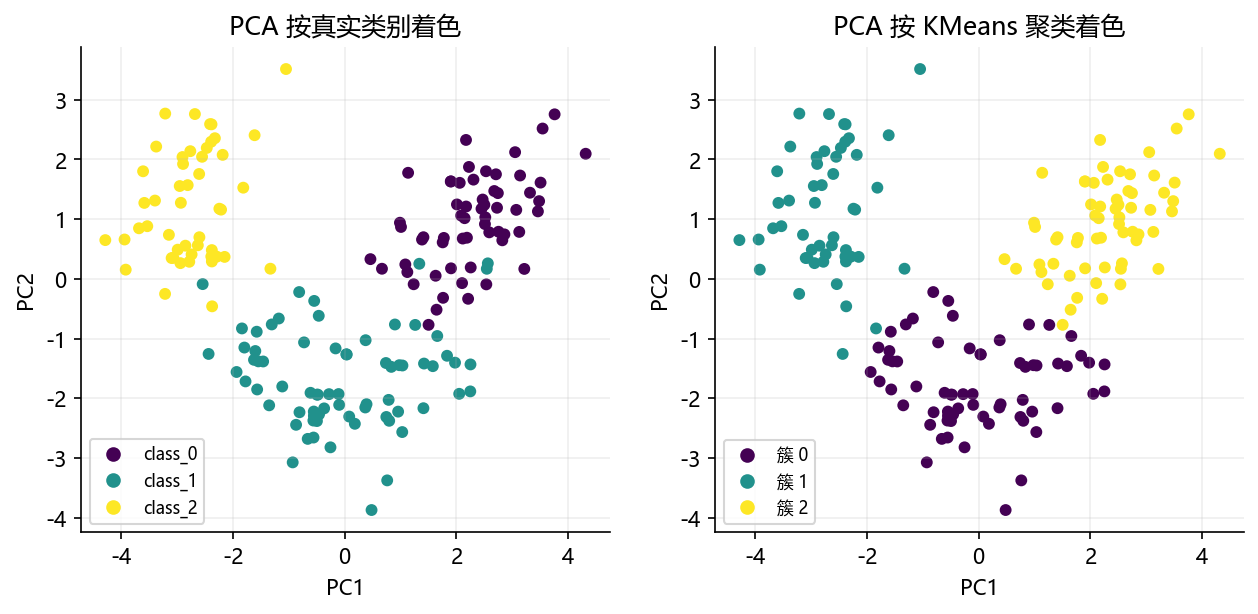
\includegraphics[keepaspectratio,alt={Wine PCA：真实类别 vs KMeans 簇}]{figures/08-sklearn/wine_pca_true_vs_kmeans.png}}
\caption{Wine PCA：真实类别 vs KMeans 簇}
\end{figure}

\begin{quote}
前两个主成分只保留约 55\% 方差，说明 13 维信息没有完全集中在 2
维，但散点已能看出三团结构；KMeans 簇与真实类别在 PCA 平面上也基本重合。
\end{quote}

\subsection{本章综合练习（上机任务）}\label{ux672cux7ae0ux7efcux5408ux7ec3ux4e60ux4e0aux673aux4efbux52a1-3}

\begin{enumerate}
\def\labelenumi{\arabic{enumi}.}
\tightlist
\item
  把本案例中的分类器换成
  \texttt{SVC}、\texttt{GradientBoostingClassifier}，比较 5 折均值。
\item
  用 \texttt{SelectKBest} 只保留前 5 个特征再分类，观察精度是否下降。
\item
  把 KMeans 的 \texttt{n\_clusters} 改为
  2、4、5，画出``k-ARI''曲线，解释最佳 k。
\item
  把 PCA 画成 2×2
  子图（PC1-PC2、PC1-PC3、PC2-PC3），观察哪个组合最易分。
\end{enumerate}

\subsection{延伸阅读}\label{ux5ef6ux4f38ux9605ux8bfb-37}

\begin{itemize}
\tightlist
\item
  sklearn 组合与
  Pipeline：https://scikit-learn.org/stable/modules/compose.html
\item
  sklearn
  特征重要性：https://scikit-learn.org/stable/modules/ensemble.html\#feature-importance
\item
  sklearn
  聚类评估（ARI/silhouette）：https://scikit-learn.org/stable/modules/clustering.html\#clustering-performance-evaluation
\end{itemize}

\section{05
常见误区与技巧}\label{ux5e38ux89c1ux8befux533aux4e0eux6280ux5de7-7}

\begin{quote}
本章新增``查漏补缺''页：把 sklearn
使用中最常见的坑集中列出，并给出性能、调试与自测清单。
\end{quote}

\subsection{1.
高频误区速查表}\label{ux9ad8ux9891ux8befux533aux901fux67e5ux8868-7}

{\def\LTcaptype{none} % do not increment counter
\begin{longtable}[]{@{}
  >{\raggedright\arraybackslash}p{(\linewidth - 6\tabcolsep) * \real{0.2500}}
  >{\raggedright\arraybackslash}p{(\linewidth - 6\tabcolsep) * \real{0.2500}}
  >{\raggedright\arraybackslash}p{(\linewidth - 6\tabcolsep) * \real{0.2500}}
  >{\raggedright\arraybackslash}p{(\linewidth - 6\tabcolsep) * \real{0.2500}}@{}}
\toprule\noalign{}
\begin{minipage}[b]{\linewidth}\raggedright
\#
\end{minipage} & \begin{minipage}[b]{\linewidth}\raggedright
误区 / 错误写法
\end{minipage} & \begin{minipage}[b]{\linewidth}\raggedright
正确做法
\end{minipage} & \begin{minipage}[b]{\linewidth}\raggedright
原因
\end{minipage} \\
\midrule\noalign{}
\endhead
\bottomrule\noalign{}
\endlastfoot
1 & \texttt{scaler.fit\_transform(X\_test)} & 训练集
\texttt{fit}，然后训练/测试都 \texttt{transform}；或用 \texttt{Pipeline}
& 用测试集统计量会``泄漏''测试信息 \\
2 & 对无序分类特征用 \texttt{LabelEncoder} & 用 \texttt{OneHotEncoder} /
\texttt{OrdinalEncoder} & 整数编码隐含顺序，误导模型 \\
3 & \texttt{r2\_score(y\_pred,\ y\_test)} &
\texttt{r2\_score(y\_test,\ y\_pred)} & 第一个参数是真值 y\_true \\
4 & 分类问题用 \texttt{r2\_score} & 用 \texttt{accuracy\_score} /
\texttt{f1\_score} / \texttt{roc\_auc\_score} & R² 只用于连续回归 \\
5 & \texttt{fit\_transform} 后再 \texttt{fit} 另一模型 & 把缩放放进
\texttt{Pipeline} 统一处理 & 避免重复/不一致的预处理 \\
6 & \texttt{load\_boston()} & 用 \texttt{load\_diabetes} /
\texttt{fetch\_california\_housing} / 自定义数据 & \texttt{load\_boston}
已在 sklearn 1.2 移除 \\
7 & \texttt{OneHotEncoder(sparse=False)} 老参数 &
\texttt{sparse\_output=False} & 新版本用 \texttt{sparse\_output} \\
8 & \texttt{RFE(estimator,\ 5)} 传位置参数 &
\texttt{RFE(estimator,\ n\_features\_to\_select=5)} & 新版
\texttt{n\_features\_to\_select} 是关键字参数 \\
9 & 用 \texttt{fit} 后直接 \texttt{transform} 新数据 & 先 \texttt{fit}
再 \texttt{transform}，否则 \texttt{NotFittedError} &
估计器必须携带训练统计量 \\
10 & \texttt{GridSearchCV} 不设 \texttt{random\_state} & 给模型与
\texttt{shuffle} 设置种子 & 结果不可复现 \\
11 & 对树模型也强制缩放 & 通常可跳过（缩放对树无益） &
树按阈值切分，不受量纲影响 \\
12 & \texttt{DBSCAN} 一个 \texttt{eps} 走天下 & 按数据量纲调
\texttt{eps}/\texttt{min\_samples} & 密度参数与数据尺度强相关 \\
13 & KMeans 不设 \texttt{random\_state} &
\texttt{KMeans(...,\ random\_state=0)} & 初始中心随机，结果不稳定 \\
14 & 用 \texttt{predict} 取概率 & 概率用
\texttt{predict\_proba}（二分类取 \texttt{{[}:,1{]}}） &
\texttt{predict} 返回类别标签 \\
15 & 混淆矩阵行/列方向记反 & 记住
\texttt{confusion\_matrix(y\_true,\ y\_pred)} 行是真值 &
行=真实，列=预测 \\
\end{longtable}
}

\subsection{2. 性能技巧}\label{ux6027ux80fdux6280ux5de7-6}

\begin{itemize}
\tightlist
\item
  \textbf{数据量优先用
  \texttt{n\_jobs=-1}}：\texttt{RandomForestClassifier(n\_jobs=-1)}、\texttt{GridSearchCV(...,\ n\_jobs=-1)}
  可并行（注意 RAM）。
\item
  \textbf{能向量化别循环}：特征处理尽量用 sklearn 方法一次性完成，避免
  Python 逐行 for。
\item
  \textbf{大矩阵用稀疏表示}：OneHot 后特征维度很大时保留稀疏矩阵（默认
  \texttt{sparse\_output=True}），别急着 \texttt{toarray()}。
\item
  \textbf{\texttt{Pipeline}
  更好维护}：把缩放、编码、特征选择、模型串成一个对象，训练/预测/调参都更安全。
\item
  \textbf{网格搜索先粗后细}：先搜大跨度，再在小范围精调；必要时用
  \texttt{RandomizedSearchCV} 代替 \texttt{GridSearchCV}。
\item
  \textbf{启用 Warm start}：增量训练可用 \texttt{partial\_fit}（如
  \texttt{SGDClassifier}）或 \texttt{warm\_start=True}（部分集成模型）。
\end{itemize}

\subsection{3. 调试建议}\label{ux8c03ux8bd5ux5efaux8bae-7}

\begin{enumerate}
\def\labelenumi{\arabic{enumi}.}
\tightlist
\item
  先打印
  \texttt{X.shape}、\texttt{y.shape}、\texttt{dtype}，确认维度与缺失值。
\item
  用 \texttt{np.isnan(X).sum()}、\texttt{np.isinf(X).sum()} 检查异常值。
\item
  出错先看 \textbf{fit 是否成功}：\texttt{model.fit(X,\ y)} 后打印
  \texttt{model.coef\_} / \texttt{model.feature\_importances\_}。
\item
  对 \texttt{Pipeline}，用 \texttt{pipe.named\_steps} 查看每一步；用
  \texttt{pipe.get\_params()} 检查参数名。
\item
  检查是否``数据泄漏''：

  \begin{itemize}
  \tightlist
  \item
    缩放器是否只 \texttt{fit} 在训练折（用 Pipeline 最保险）；
  \item
    \texttt{train\_test\_split} 是否在归一化之前。
  \end{itemize}
\item
  收敛警告（如``lbfgs failed to
  converge''）通常提示：特征未缩放、\texttt{max\_iter}
  太小，或类别不平衡。
\item
  固定所有随机种子（\texttt{random\_state}）并记录，便于复现与讨论。
\end{enumerate}

\subsection{4.
本章小结（自测）}\label{ux672cux7ae0ux5c0fux7ed3ux81eaux6d4b-4}

\begin{itemize}
\tightlist
\item[$\square$]
  能说清 \texttt{fit} / \texttt{transform} / \texttt{fit\_transform}
  的区别；
\item[$\square$]
  能用 Pipeline 做``缩放 + 模型''，避免数据泄漏；
\item[$\square$]
  能区分分类（准确率/F1/AUC）与回归（MSE/MAE/R²）指标；
\item[$\square$]
  能解释 \texttt{StandardScaler} 与 \texttt{MinMaxScaler} 的差异；
\item[$\square$]
  能比较 KMeans 与 DBSCAN 的适用场景；
\item[$\square$]
  能用 PCA / LDA 降到 2 维并读 \texttt{explained\_variance\_ratio\_}；
\item[$\square$]
  能独立完成 04 综合案例并写 3 句结论。
\end{itemize}

\subsection{延伸阅读}\label{ux5ef6ux4f38ux9605ux8bfb-38}

\begin{itemize}
\tightlist
\item
  sklearn API 速查：https://scikit-learn.org/stable/modules/classes.html
\item
  sklearn
  常见陷阱（用户指南）：https://scikit-learn.org/stable/modules/preprocessing.html
\item
  sklearn
  调试/性能相关：https://scikit-learn.org/stable/developers/performance.html
\end{itemize}

\backmatter
